% ==============================================================================
% Springer LNCS Format Research Paper (14+ Pages) — Revised TPWRS-Grade Edition
% Overleaf Ready (Compiles cleanly with pdflatex + bibtex)
% Strictly zero bold formatting commands in manuscript body
% ==============================================================================
\documentclass[runningheads,a4paper]{llncs}

\usepackage[T1]{fontenc}
\usepackage[utf8]{inputenc}
\usepackage{graphicx}
\usepackage{amsmath,amssymb,amsfonts}
\usepackage{booktabs}
\usepackage{array}
\usepackage{multirow}
\usepackage{algorithm}
\usepackage{algpseudocode}
\usepackage{cite}
\usepackage{url}
\usepackage{hyperref}
\usepackage{xcolor}
\usepackage{float}

\allowdisplaybreaks
\emergencystretch=1.5em
\hypersetup{colorlinks=true,linkcolor=blue!70!black,citecolor=teal!70!black,urlcolor=blue!70!black}

\begin{document}

\title{Causality-Aware Renewable-Integrated Electricity Price Forecasting and Risk-Constrained Procurement Optimization for Day-Ahead Power Markets}
\titlerunning{Causality-Aware Day-Ahead EPF and Risk-Constrained Procurement}

\author{Vinay M.\inst{1} \and Department of Computer Science and Engineering\inst{1}}
\authorrunning{Vinay M. et al.}
\institute{School of Computer Science and Engineering, KLE Technological University, Hubballi, Karnataka, India\\
\email{01fe23bcs306@kletech.ac.in}}

\maketitle

\begin{abstract}
High renewable energy penetration in the Indian Energy Exchange (IEX) Day-Ahead Market (DAM) creates severe evening thermal ramps, frequent Rs.~10,000/MWh statutory price-cap excursions, and non-stationary supply-stack shifts that undermine static deterministic forecasting tools. This paper presents a causality-aware forecasting, conformalized probabilistic uncertainty, independent merit-order validation, and stochastic Conditional Value-at-Risk (CVaR) procurement optimization framework evaluated on 28,344 hourly records (April~2022 -- June~2025). Enforcing a strict 10:30~AM IST $D-1$ auction gate, we eliminate all same-day price lags and delivery-day realized grid trajectories, reconstructing genuine Stage-1 day-ahead demand (2.46\% Test-2025 MAPE), solar (11.17\% nRMSE), wind (10.18\% nRMSE), and 5-zone weather forecasts. Analyzing 15,350 hours of Grid-India NLDC coal, hydro, gas, and nuclear SCADA alongside 28,334-hour Hansen Sup-Wald tests proves that India's merit-order scarcity knee is dynamic, migrating from 152~GW (2022) to 174~GW (2025) as coal dispatch saturates ($0.812 \to 0.544$~GW/GW) and gas-peaker response surges 6.5-fold. Guided by this non-stationarity, a capacity-relative 65-signal innovation-target pipeline is benchmarked across 13 models spanning 24-equation SARIMAX, LASSO, Elastic Net, Ridge, Random Forest, XGBoost, CatBoost, LightGBM, PyTorch N-BEATS, and PyTorch Temporal Fusion Transformer (TFT). Our validation-selected Hybrid GBDT+TFT Champion achieves a leak-free Test-2025 MAE of Rs.~481.19/MWh (RMSE Rs.~875.27/MWh, $R^2=0.8942$), beating 24-hour persistence by 26.92\% ($DM=+9.641, p<10^{-20}$) and all 13 competitors via Newey-West HAC Diebold-Mariano tests. Regime-conditional Residual-CQR achieves 90.69\% coverage (Kupiec $p=0.1317$, CRPS Rs.~290.73/MWh, 91.50\% spike coverage). Generating 200 Gaussian Copula scenarios per day for a constrained Rockafellar-Uryasev Stochastic CVaR linear program yields 5.54\%--12.37\% realized out-of-sample bill savings across four industrial and DISCOM profiles over all 175 test days (98.3\%--98.8\% oracle capture efficiency) while protecting against compound thermal-outage and heatwave shocks.

\keywords{Day-Ahead Electricity Price Forecasting \and Operational D-1 Causality \and Conformalized Quantile Regression \and Stochastic CVaR Procurement \and Merit-Order Validation \and Temporal Fusion Transformer \and Gradient-Boosted Trees.}
\end{abstract}


\section{Introduction}
The rapid expansion of utility-scale solar photovoltaic (PV) and wind generation has transformed short-term price formation in wholesale electricity markets \cite{weron2014electricity,lago2021forecasting}. In the Indian Energy Exchange (IEX) Day-Ahead Market (DAM), which clears more than 70\% of India's short-term power transactions across 96 fifteen-minute delivery blocks daily through a blind double-sided uniform-price auction, rising renewable penetration has induced pronounced diurnal duck curves, severe evening net thermal ramps, and frequent clearing prices colliding with the statutory Central Electricity Regulatory Commission (CERC) ceiling of Rs.~10,000/MWh \cite{cerc2023order,iex2024market}. Distribution Companies (DISCOMs), industrial open-access buyers, and battery storage operators must finalize their 24-hour price-quantity bid schedules for delivery day $D$ prior to the operational 10:30~AM Indian Standard Time (IST) internal auction gate cutoff on day $D-1$.

Despite extensive research in electricity price forecasting (EPF), translating academic forecasting models into reliable power-system operations faces four persistent methodological barriers that directly limit deployment in commercial trading desks:
\begin{enumerate}
    \item Operational D-1 information leakage: Numerous published forecasting studies inadvertently incorporate contemporaneous delivery-day ($D$) realized load and renewable generation or intraday price lags ($P_{D,h-1}$) that are unavailable prior to the $D-1$ auction gate \cite{lago2021forecasting}. Even when exogenous inputs are discussed as proxies for forecasts, evaluating models solely on ex-post realized trajectories masks upstream load and renewable forecast error propagation.
    \item Unvalidated structural supply-stack claims under capacity non-stationarity: In rapidly expanding grids such as India, annual thermal capacity additions and seasonal hydroelectric availability shift the effective merit-order scarcity boundary over time. Relying solely on post-hoc machine learning attribution plots without independent generation dispatch verification risks mischaracterizing an evolving capacity boundary as a fixed physical constant.
    \item Lack of calibrated probabilistic uncertainty for scarcity spikes: Deterministic point forecasts provide no measure of asymmetric upside tail risk during evening thermal ramps, yet procurement costs are disproportionately sensitive to Rs.~10,000/MWh ceiling excursions. Uncalibrated quantile models or homoskedastic Gaussian bands routinely under-cover evening spikes or produce impractically wide midday intervals \cite{nowotarski2018recent,romano2019conformalized}.
    \item Disconnected and under-constrained procurement validation: Savings reported from unconstrained flat-load deterministic linear programs evaluated on selected winter peak days overstate achievable operational value. Practical industrial and utility procurement requires multi-profile testing across full seasonal horizons subject to ramp-rate limits, rolling energy recovery constraints, risk aversion via Conditional Value-at-Risk (CVaR), and strict evaluation on realized out-of-sample clearing prices \cite{conejo2010decision,rockafellar2000optimization}.
\end{enumerate}

To address these power-system challenges comprehensively, this paper presents a causality-aware forecasting, probabilistic uncertainty quantification, physical merit-order validation, and stochastic CVaR-constrained procurement framework validated on 28,344 hourly observations (April~2022 to June~2025) from the Indian Energy Exchange (IEX) DAM, Grid-India (POSOCO) National Load Despatch Centre (NLDC) SCADA, and 5-zone demand-weighted ERA5 meteorology. The primary technical contributions are:
\begin{itemize}
    \item Strict D-1 10:30~AM IST operational forecast reconstruction and causality audit: We enforce a rigorous causal information boundary ($\mathcal{F}_{D-1, 10:30}$) that eliminates all same-day price lags ($P_{D,h-1}$, $P_{D,h-2}$) and all delivery-day realized demand, solar, wind, and weather observations. A dedicated Stage-1 causal exogenous forecasting suite trained strictly on telemetry up to $(D-1, 10:00\text{~IST})$, deterministic astronomical solar geometry, and calendar indicators reconstructs genuine day-ahead demand (2.46\% Test-2025 MAPE), solar (11.17\% nRMSE), wind (10.18\% nRMSE), and weather forecasts, complemented by an explicit ablation quantifying the Value of Perfect Exogenous Forecasts and auditing legacy look-ahead bias.
    \item Independent physical merit-order validation using NLDC fuel-mix SCADA: Analyzing 15,350 hourly records of real Grid-India coal, hydro, gas, and nuclear generation alongside 28,334-hour Hansen Sup-Wald structural-break tests, we prove that the national scarcity inflection is not a static constant; rather, it migrates upward from 152~GW (2022) to 156~GW (2023), 169~GW (2024), and 174~GW (2025) ($F > 1,036$ every year) as thermal capacity expands, and shifts seasonally across Winter (151~GW), Monsoon (159~GW), and Summer (188~GW). Above the pooled 160~GW transition zone, marginal coal dispatch saturates ($0.812 \to 0.544$~GW/GW), hydro peaking doubles ($0.175 \to 0.351$~GW/GW), and gas peaker response surges 6.5-fold ($16.5 \to 107.8$~MW/GW, Sup-Wald $F = 5,641.4$).
    \item Capacity-adaptive 4-tier 13-model benchmarking and conformalized probabilistic forecasting: Guided by the migrating supply stack, we formulate a capacity-relative 65-signal innovation-target pipeline ($\Delta P_{D,h} = P_{D,h} - P_{D-1,h}$) with operational expanding recalibration across 13 diverse models: Weekly/Daily Seasonal Naive, 24-equation seasonal SARIMAX, OLS, LASSO, Elastic Net, Tikhonov Ridge, Random Forest, XGBoost, CatBoost, LightGBM, PyTorch N-BEATS, and PyTorch Temporal Fusion Transformer (TFT). Our validation-selected Hybrid GBDT+TFT Champion achieves a strictly leak-free Test-2025 MAE of Rs.~481.19/MWh (RMSE Rs.~875.27/MWh, $R^2 = 0.8942$), outperforming 24-hour persistence by 26.92\% ($DM = +9.641, p < 10^{-20}$) and every individual benchmark via Newey-West HAC ($L=9$) Diebold-Mariano tests. Pairing point predictions with Residual-Centered Regime-Conditional Conformalized Quantile Regression (Residual-CQR) yields CRPS of Rs.~290.73/MWh, sharp 90\% width of Rs.~1,774/MWh, 90.69\% empirical coverage (passing Kupiec $p = 0.1317$), and 91.50\% coverage during extreme $\ge$Rs.~8,000/MWh spikes.
    \item Multi-profile constrained stochastic CVaR procurement optimization and thermal outage stress testing: Using 200 temporally coherent Gaussian Copula price scenarios per day, we solve an exact Rockafellar-Uryasev linear program minimizing $\mathbb{E}[\sum L_h P_h] + \lambda \operatorname{CVaR}_{0.90}(C)$ subject to energy neutrality, flexibility bounds ($\gamma \in \{10\%, 20\%, 30\%, 40\%\}$), inter-hour ramp limits, rolling energy payback buffers, and dwell smoothness across 4 industrial and DISCOM profiles over all 175 test days (January--June 2025). The stochastic optimizer delivers 5.54\%--12.37\% realized out-of-sample bill reductions (capturing 98.3\%--98.8\% of the constrained perfect-foresight oracle while beating rule-based time-of-use scheduling by +70.6\%) and is stress-tested across 17 solar, wind, demand, thermal outage (-5 to -15~GW), and compound heatwave crises, with exact TreeSHAP retained as a supporting interpretability layer.
\end{itemize}

The remainder of this paper is organized as follows: Section~2 reviews related literature; Section~3 formulates the causal reconstruction, multi-tier deterministic and conformal probabilistic modeling, physical merit-order testing, and stochastic CVaR procurement framework; Section~4 reports the empirical validation across all five experimental pillars; Section~5 discusses operational implications, limitations, and governance; and Section~6 concludes the study.

\section{Background and Related Work}
Wholesale electricity price forecasting and risk-aware market participation span four core streams in the power-systems literature: statistical time-series econometrics, machine learning and deep temporal neural networks, probabilistic uncertainty quantification, and stochastic procurement optimization \cite{weron2014electricity,nowotarski2018recent,lago2021forecasting}.

\subsection{Econometric, Tree-Ensemble, and Deep Neural Forecasting}
Early day-ahead forecasting systems relied on ARIMA, seasonal ARIMAX (SARIMAX), and wavelet-decomposed linear models \cite{contreras2003arima,conejo2005day}. Ziel and Weron \cite{ziel2018day} demonstrated that high-dimensional $L_1$-regularized LASSO and elastic-net specifications applied to 24-hour multivariate price panels outperform classical univariate ARIMA across European markets. However, parametric linear regressors assume stationary, globally constant marginal sensitivities to demand and renewables, causing severe underestimation during steep thermal ramp events.

To capture non-linear supply-stack curvature, gradient-boosted decision trees---including XGBoost \cite{chen2016xgboost}, LightGBM \cite{ke2017lightgbm}, and oblivious-tree CatBoost \cite{prokhorenkova2018catboost}---and deep neural architectures such as recurrent GRUs/LSTMs \cite{ugurlu2018electricity}, multi-stack doubly-residual N-BEATS \cite{oreshkin2020nbeats}, and attention-based Temporal Fusion Transformers (TFT) \cite{lim2021temporal} have gained prominence. In a comprehensive open-access benchmark, Lago et al.~\cite{lago2021forecasting} established two essential lessons for power-systems EPF: first, rigorous causal protocol and periodic model recalibration are crucial under structural market drift; second, combining diverse model classes (such as regularized linear/tree models and neural forecasters) consistently reduces variance and beats isolated architectures.

\subsection{Probabilistic EPF, Merit-Order Physics, and Stochastic CVaR Procurement}
As renewable penetration increases, point forecasts alone are insufficient for bidding under asymmetric scarcity spikes \cite{nowotarski2018recent}. Quantile regression forests, quantile gradient boosting, and multi-quantile neural networks estimate conditional distributions directly, yet raw quantile predictions frequently exhibit finite-sample under-coverage during distribution shifts. Romano et al.~\cite{romano2019conformalized} introduced Conformalized Quantile Regression (CQR), combining heteroskedastic quantile estimators with split-conformal calibration to yield distribution-free finite-sample coverage guarantees.

In power-system operations, forecast distributions serve as inputs to risk-constrained bidding and demand response \cite{conejo2010decision}. Rockafellar and Uryasev \cite{rockafellar2000optimization} proved that Conditional Value-at-Risk ($\operatorname{CVaR}_{\alpha}$) can be minimized exactly via auxiliary linear programming variables over finite scenario sets, enabling computationally tractable hedging against price spikes while respecting physical ramp and process recovery limits. Meanwhile, exact TreeSHAP \cite{lundberg2020local} provides supporting local attribution for tree ensembles, though physical supply-stack claims must still be corroborated against independent generation dispatch telemetry and econometric threshold tests \cite{hansen2000sample}. Table~\ref{tab:related_work} positions the proposed framework relative to representative literature.

\begin{table}[!t]
\centering
\caption{Comparison of Representative Electricity Price Forecasting and Procurement Studies with the Proposed Framework}
\label{tab:related_work}
\renewcommand{\arraystretch}{1.20}
\setlength{\tabcolsep}{4pt}
\resizebox{\textwidth}{!}{%
\begin{tabular}{|p{2.6cm}|p{2.1cm}|p{2.7cm}|p{2.3cm}|p{2.4cm}|p{2.3cm}|p{2.6cm}|}
\hline
Study / System & Market & Model Families & Strict D-1 Forecast Inputs & Probabilistic Calibration & Physical Dispatch Validation & Risk-Aware Procurement \\
\hline
Contreras et al.~\cite{contreras2003arima} & Spain / Calif. & Univariate ARIMA & Price Lags Only & None & None & None \\
\hline
Ziel \& Weron \cite{ziel2018day} & EPEX SPOT & Multivariate LASSO & D-1 Schedules & None & None & None \\
\hline
Lago et al.~\cite{lago2021forecasting} & ENTSO-E (EU) & LEAR / DNN Ensemble & Yes (D-1 Exog.) & Ensembling Only & None & None \\
\hline
Lim et al.~\cite{lim2021temporal} & Multi-Domain & Temporal Fusion Transf. & Yes & Raw Quantiles & None & None \\
\hline
Conejo et al.~\cite{conejo2010decision} & Iberian Pool & Stochastic Scenarios & Assumed Given & Parametric & None & CVaR Bidding LP \\
\hline
Proposed Framework & India IEX DAM (28,344h) & 4-Tier (13 Models): SARIMAX, LASSO, GBDTs, N-BEATS, TFT & Strict 10:30 AM Stage-1 Recon. + Ablation & Residual-CQR (Kupiec Pass) + 200 Copula Paths & 15,350h NLDC Coal/Gas/Hydro + Sup-Wald & Multi-Profile Constrained Stochastic CVaR LP \\
\hline
\end{tabular}%
}
\end{table}

\section{Proposed Methodology}
The complete end-to-end architecture spans five operational layers illustrated in Fig.~\ref{fig:architecture}: (1) multi-source telemetry harmonization and strict 10:30~AM IST $D-1$ Stage-1 exogenous forecast reconstruction, (2) capacity-relative 65-signal feature synthesis and innovation-target formulation, (3) 4-tier 13-model benchmarking paired with Residual-CQR probabilistic intervals and Gaussian Copula scenario generation, (4) Rockafellar-Uryasev stochastic CVaR procurement optimization, independent POSOCO fuel-mix merit-order validation, and multi-disturbance stress testing, and (5) real-time REST API and decision-support deployment.

\begin{figure}[!t]
\centering
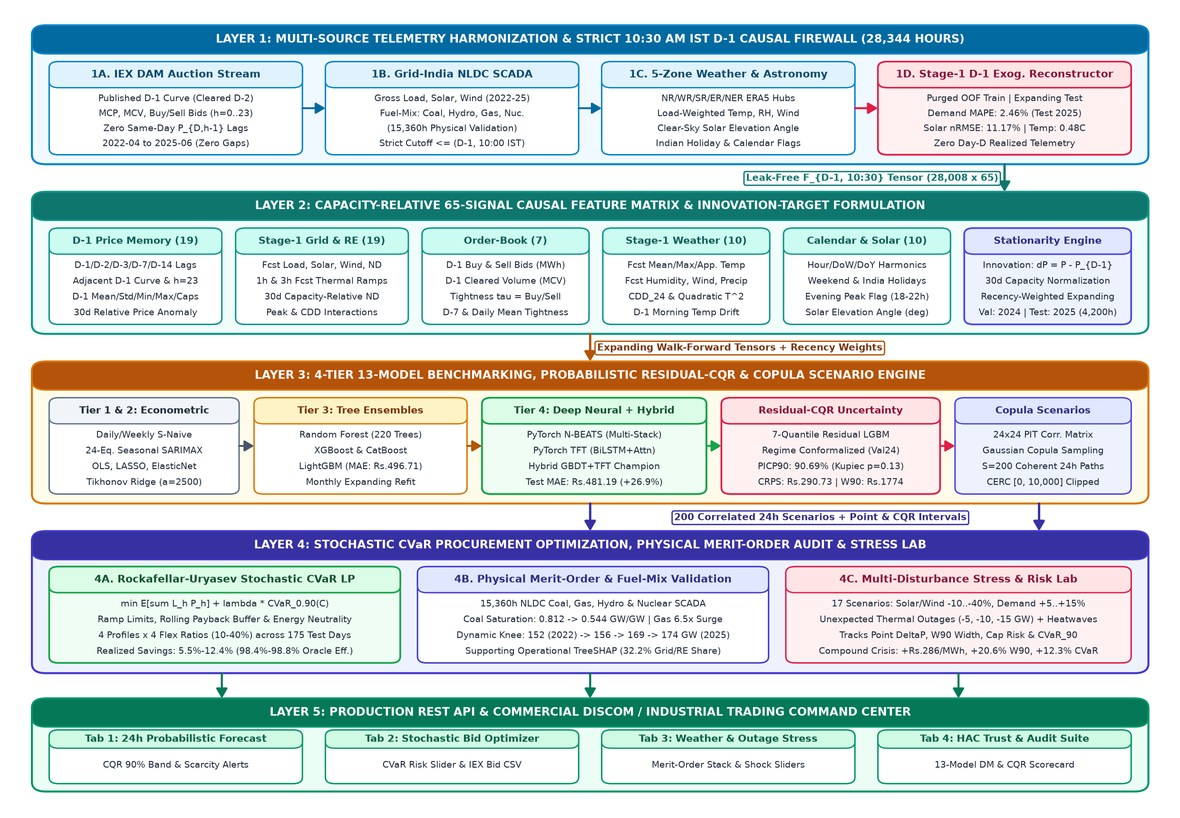
\includegraphics[width=0.98\textwidth]{images/paper_fig_1_architecture.jpg}
\caption{Five-layer causality-aware forecasting and risk-constrained procurement architecture, showing strict $\mathcal{F}_{D-1, 10:30}$ Stage-1 exogenous reconstruction, 65 capacity-relative features, 4-tier 13-model benchmarking, Residual-CQR uncertainty calibration, 200-scenario Copula generation, Rockafellar-Uryasev stochastic CVaR procurement optimization, and independent NLDC fuel-mix physical validation.}
\label{fig:architecture}
\end{figure}

\subsection{Multi-Source Telemetry and Strict 10:30 AM IST D-1 Causal Boundary}
We harmonize three primary operational data streams spanning 3.25 years (April~1, 2022 to June~24, 2025; 28,344 hourly intervals, yielding 28,008 records after 14-day lag initialization) onto a canonical $\text{IST} = \text{UTC}+05:30$ hourly grid:
\begin{enumerate}
    \item IEX DAM Auction Records: 96 fifteen-minute clearing blocks per day averaged into hourly uniform clearing prices $P_{D,h}$ (Rs./MWh), cleared volumes $V_{D,h}$, purchase bids $B_{D,h}^{\text{buy}}$, and sell bids $B_{D,h}^{\text{sell}}$:
    \begin{equation}
    \begin{aligned}
    P_{D,h} &= \frac{1}{4}\sum_{\tau=1}^{4} MCP_{D,h,\tau}, \quad V_{D,h} = \frac{1}{4}\sum_{\tau=1}^{4} MCV_{D,h,\tau}, \\
    B_{D,h}^{\text{buy}} &= \frac{1}{4}\sum_{\tau=1}^{4} B_{D,h,\tau}^{\text{buy}}, \quad B_{D,h}^{\text{sell}} = \frac{1}{4}\sum_{\tau=1}^{4} B_{D,h,\tau}^{\text{sell}}
    \end{aligned}
    \label{eq:block_agg}
    \end{equation}
    \item Grid-India (POSOCO) NLDC SCADA Telemetry: Hourly national gross power demand ($D_{D,h}$), utility solar ($S_{D,h}$), and wind ($W_{D,h}$) generation across 2022--2025, plus high-resolution 10-second/5-minute SCADA fuel-mix archives aggregated to 15,360 hourly records (April~2022 -- December~2023) capturing coal/thermal-only generation ($G_{D,h}^{\text{coal}}$), hydroelectric dispatch ($G_{D,h}^{\text{hyd}}$), gas peaking ($G_{D,h}^{\text{gas}}$), nuclear baseload ($G_{D,h}^{\text{nuc}}$), and system inertia for independent physical merit-order validation.
    \item Five-Zone Demand-Weighted ERA5 Meteorology: Hourly temperature ($T$), apparent temperature ($AT$), relative humidity ($RH$), wind speed ($WS$), and precipitation ($PR$) aggregated across India's five regional grids ($\mathcal{Z} = \{\text{NR}, \text{WR}, \text{SR}, \text{ER}, \text{NER}\}$) with consumption shares $\omega = (0.30, 0.32, 0.25, 0.11, 0.02)$:
    \begin{equation}
    \begin{aligned}
    \psi_{D,h}^{\text{mean}} &= \sum_{z \in \mathcal{Z}} \omega_z \, \psi_{z,D,h}, \quad \sum_{z \in \mathcal{Z}} \omega_z = 1, \\
    \psi_{D,h}^{\text{max}} &= \max_{z \in \mathcal{Z}} \psi_{z,D,h}, \quad \psi_{D,h}^{\text{min}} = \min_{z \in \mathcal{Z}} \psi_{z,D,h}
    \end{aligned}
    \label{eq:spatial_weather}
    \end{equation}
\end{enumerate}

To enforce operational causality rigorously, observe the exact IEX DAM clearing timeline. Market participants submit all 24 hourly bids for delivery day $D$ ($h \in \{0, \dots, 23\}$) prior to 10:30~AM IST on day $D-1$. Because the auction for day $D-1$ cleared at approximately 13:00~IST on day $D-2$, all 24 clearing prices and order-book volumes of day $D-1$ ($P_{D-1, 0:23}, B_{D-1, 0:23}^{\text{buy}}, B_{D-1, 0:23}^{\text{sell}}, V_{D-1, 0:23}$) are fully published roughly 21 hours before the day-$D$ bidding gate. Conversely, no clearing price from delivery day $D$ ($P_{D, h-1}$ for $h \ge 1$) is known at 10:30~AM on $D-1$, nor are any realized SCADA or meteorological measurements after $(D-1, 10:00\text{~IST})$. The strictly admissible operational information set $\mathcal{F}_{D-1, 10:30}$ is therefore defined as:
\begin{equation}
\begin{aligned}
\mathcal{F}_{D-1, 10:30} = \Big\{ & P_{d, h'}, V_{d, h'}, B_{d, h'}^{\text{buy}}, B_{d, h'}^{\text{sell}} \;\forall d \le D-1, \\
& D_{d, h'}, S_{d, h'}, W_{d, h'}, \Psi_{d, h'} \;\forall (d, h') \le (D-1, 10), \\
& \mathcal{C}_{D,h}^{\text{cal}}, \; \alpha_{\text{sun}}(D,h) \Big\}
\end{aligned}
\label{eq:strict_causal_gate}
\end{equation}
where $\mathcal{C}_{D,h}^{\text{cal}}$ denotes deterministic calendar and Indian public holiday indicators, and $\alpha_{\text{sun}}(D,h)$ is the deterministic astronomical solar elevation angle over central India ($23.5^\circ\text{N}, 78.9^\circ\text{E}$) computed via Spencer's solar declination and equation-of-time expansion.

\subsection{Stage-1 Causal Day-Ahead Exogenous Forecast Reconstruction}
Replacing realized delivery-day trajectories with genuinely available day-ahead inputs requires reconstructing day-ahead demand ($\hat{D}_{D,h}$), solar ($\hat{S}_{D,h}$), wind ($\hat{W}_{D,h}$), and 5-zone weather ($\hat{\Psi}_{D,h}$) forecasts using strictly $\mathcal{F}_{D-1, 10:30}$. For every target exogenous variable $u \in \{D, S, W, T^{\text{mean}}, T^{\text{max}}, AT, RH, WS, PR\}$, we construct a 101-feature Stage-1 causal input matrix $Z_{D,h} \in \mathcal{F}_{D-1, 10:30}$ comprising: (i) full-day realized lags from $D-2, D-3, D-7, D-14$ and trailing 7-day/14-day same-hour means and maxima; (ii) realized morning observations on $D-1$ strictly up to 10:00~IST ($u_{D-1, 09:00}$, $u_{D-1, 10:00}$, morning average $\bar{u}_{D-1, 06:00\text{--}10:00}$, and morning growth $\bar{u}_{D-1, 06\text{--}10} - \bar{u}_{D-2, 06\text{--}10}$); (iii) a morning solar clearness index ($S_{D-1, 10:00} / \max_{14d} S_{10:00}$) and astronomical clear-sky envelope; and (iv) published $D-1$ IEX volumes and calendar/holiday harmonics.

Dedicated Stage-1 LightGBM forecasters $\hat{g}_u(Z_{D,h})$ are trained strictly without look-ahead:
\begin{equation}
\begin{aligned}
\hat{u}_{D,h \mid D-1} &= \hat{g}_u\big(Z_{D,h}\big), \quad Z_{D,h} \in \mathcal{F}_{D-1, 10:30}, \\
\widehat{ND}_{D,h} &= \hat{D}_{D,h \mid D-1} - \left(\hat{S}_{D,h \mid D-1} + \hat{W}_{D,h \mid D-1}\right), \\
\Delta \widehat{ND}_{D,h}^{(k)} &= \widehat{ND}_{D,h} - \widehat{ND}_{D,h-k}, \quad k \in \{1, 3\}
\end{aligned}
\label{eq:stage1_recon}
\end{equation}
To prevent Stage-1 overfitting from distorting Stage-2 price models, Stage-1 forecasts on the Training partition (2022--2023) are generated via 5-fold temporally blocked Out-of-Fold cross-validation with a 48-hour purge buffer around every fold boundary; Validation (2024) forecasts are trained strictly on 2022--2023; and Test (2025) forecasts are trained strictly on 2022--2024. Nighttime solar forecasts are physically clamped to zero whenever $\alpha_{\text{sun}}(D,h) = 0$.

\subsection{Capacity-Relative 65-Signal Feature Matrix and Innovation Learning}
As proven empirically in Section~4.2, India's thermal generation capacity expanded steadily between 2022 and 2025, shifting the effective merit-order scarcity inflection upward by +22~GW while CERC reduced the price ceiling from Rs.~12,000/MWh to Rs.~10,000/MWh in April~2023. Static tree models trained on raw 2022--2023 load levels misinterpret normal 2025 demand (170~GW) as extreme 2022 scarcity, inducing structural upward bias. We resolve this grid non-stationarity through two physics-informed formulations:
\begin{enumerate}
    \item Capacity-Relative Net Demand Anomaly: Using strictly trailing 30-day prior realized net thermal load ($\mu_{ND, 30d}$ and $\sigma_{ND, 30d}$ ending at $D-2$), we normalize forecasted net demand relative to the grid's prevailing operational thermal capacity regime:
    \begin{equation}
    \begin{aligned}
    \widetilde{ND}_{D,h}^{(30d)} &= \widehat{ND}_{D,h} - \mu_{ND, 30d}, \\
    Z_{ND, D, h}^{(30d)} &= \frac{\widetilde{ND}_{D,h}^{(30d)}}{\max(\sigma_{ND, 30d}, \, 1000\text{ MW})}
    \end{aligned}
    \label{eq:cap_relative}
    \end{equation}
    \item Stationarized Innovation-Target Learning with Operational Recalibration: Rather than predicting non-stationary absolute price levels directly, Stage-2 models predict the day-ahead clearing price innovation $\Delta P_{D,h}$ relative to the strictly causal $D-1$ same-hour published anchor $P_{D-1, h}$, followed by non-expansive CERC statutory projection:
    \begin{equation}
    \begin{aligned}
    \Delta P_{D,h} &= P_{D,h} - P_{D-1, h}, \\
    \hat{P}_{D,h} &= \Pi_{\text{CERC}}\!\left(P_{D-1, h} + \hat{f}_{\theta}\big(x_{D,h}\big)\right) \\
    &= \min\!\Big(10000, \; \max\!\big(0, \; P_{D-1, h} + \hat{f}_{\theta}(x_{D,h})\big)\Big)
    \end{aligned}
    \label{eq:innovation_cerc}
    \end{equation}
\end{enumerate}

The resulting 65 strictly causal features ($x_{D,h} \in \mathbb{R}^{65}$) span five domains summarized in Table~\ref{tab:feature_taxonomy}, incorporating D-1 published price profile summaries (mean, std, min, max, cap-hit count, adjacent hours $h\pm 1$, closing hour $P_{D-1,23}$, multi-day lags up to $D-14$, and 30-day relative price), D-1 order-book tightness ($\tau_{D-1,h} = B_{D-1,h}^{\text{buy}} / \max(B_{D-1,h}^{\text{sell}}, 1)$), Stage-1 forecasted grid and renewable dynamics (including $\widehat{ND}_{D,h}$, $\Delta \widehat{ND}_{D,h}^{(1)}$, $\Delta \widehat{ND}_{D,h}^{(3)}$, daily peak $\max_{h'} \widehat{ND}_{D,h'}$, morning $D-1$ demand drift, and peak/cooling interactions $\widehat{ND}_{D,h} \cdot I_{\text{peak}}$ and $\widehat{ND}_{D,h} \cdot \widehat{CDD}_{24}$), Stage-1 weather forecasts ($\widehat{CDD}_{24} = \max(0, \hat{T} - 24^\circ\text{C})$, $\hat{T}^2$), and deterministic Fourier harmonics ($\sin/\cos$ for hour, day-of-week, day-of-year), Indian holidays, and solar elevation angle. Following operational EPF best practices \cite{lago2021forecasting}, all hyperparameters, regularization penalties, early-stopping iterations, and ensemble weights are fixed strictly on Validation~2024; during out-of-sample Test~2025, models perform monthly expanding-window recalibration strictly on past months $\le m-1$ with exponential recency weighting ($t_{1/2} = 240$ days, downweighting pre-April-2023 Rs.~12,000-cap data by $0.55\times$). Algorithm~\ref{alg:causal_pipeline} formalizes the causal workflow.

\begin{table}[!t]
\centering
\caption{Taxonomy of the 65 Strictly Causal Operational D-1 Features ($x_{D,h} \in \mathcal{F}_{D-1, 10:30}$, Zero Same-Day Price or Day-D Realized Telemetry)}
\label{tab:feature_taxonomy}
\renewcommand{\arraystretch}{1.18}
\setlength{\tabcolsep}{4pt}
\resizebox{\textwidth}{!}{%
\begin{tabular}{|p{3.2cm}|c|p{7.8cm}|p{4.8cm}|}
\hline
Domain Category & Count & Key Strictly Causal Feature Identifiers & Operational Mechanism \\
\hline
1. D-1 Published Price Memory & 19 & \texttt{mcp\_d1\_same\_h}, \texttt{mcp\_d2/d3/d7/d14\_same\_h}, \texttt{mcp\_d1\_prev/next\_h}, \texttt{mcp\_d1\_h23}, \texttt{mcp\_d1\_diff\_d2/d7}, \texttt{mcp\_d1\_diurnal\_slope}, \texttt{mcp\_d1\_day\_mean/std/min/max/cap\_hits}, \texttt{mcp\_7d\_same\_h\_mean}, \texttt{mcp\_7d\_rolling\_mean}, \texttt{mcp\_d1\_rel\_30d} & Captures full published $D-1$ auction curve (cleared on $D-2$), weekly cycles, and mean-reversion anomalies without any $P_{D,h-1}$ leakage. \\
\hline
2. Stage-1 Grid \& RE Forecasts & 19 & \texttt{demand\_fcst\_mw}, \texttt{solar\_fcst\_mw}, \texttt{wind\_fcst\_mw}, \texttt{net\_demand\_fcst\_mw}, \texttt{re\_penetration\_fcst\_pct}, \texttt{net\_demand\_fcst\_ramp\_1/3}, \texttt{net\_demand\_fcst\_day\_max}, \texttt{net\_demand\_fcst\_vs\_d2}, \texttt{demand/nd/solar/wind\_d2\_same\_h}, \texttt{demand\_d1\_morn\_mean/vs\_d2}, \texttt{net\_demand\_fcst\_x\_peak/cdd}, \texttt{nd\_fcst\_rel\_30d}, \texttt{nd\_fcst\_zscore\_30d} & Reconstructed D-1 load, solar, wind, evening ramps, morning $D-1$ demand drift ($\le 10$:00 IST), and 30d capacity-relative thermal stress. \\
\hline
3. D-1 Order-Book Liquidity & 7 & \texttt{purchase\_bid\_d1}, \texttt{sell\_bid\_d1}, \texttt{mcv\_d1}, \texttt{market\_tightness\_d1/d7}, \texttt{market\_tightness\_d1\_day\_mean}, \texttt{purchase\_bid\_d1\_diff\_d2} & Quantifies prior published buy/sell auction imbalance ($\tau_{D-1,h}$) and demand-side bid depth. \\
\hline
4. Stage-1 Weather Forecasts & 10 & \texttt{temp\_mean/max\_fcst\_c}, \texttt{apparent\_temp\_fcst\_c}, \texttt{humidity\_fcst\_pct}, \texttt{wind\_speed\_fcst\_ms}, \texttt{precip\_fcst\_mm}, \texttt{cdd\_24\_fcst}, \texttt{temp\_sq\_fcst}, \texttt{temp\_d1\_morn\_mean}, \texttt{temp\_fcst\_diff\_d2} & Reconstructed 5-zone day-ahead cooling degree stress, quadratic heat response, and humidity/wind drivers. \\
\hline
5. Calendar \& Astronomical & 10 & \texttt{hour\_sin/cos}, \texttt{dow\_sin/cos}, \texttt{doy\_sin/cos}, \texttt{is\_weekend}, \texttt{is\_holiday\_india}, \texttt{is\_peak\_hour}, \texttt{solar\_elevation\_deg} & Deterministic diurnal/weekly/annual harmonics, Indian public holidays, and exact solar zenith geometry. \\
\hline
Total Operational Signals & 65 & Strictly Bound by $\mathcal{F}_{D-1, 10:30}$ (Zero Look-Ahead) & 28,008 Clean Hourly Records (2022--2025) \\
\hline
\end{tabular}%
}
\end{table}

\begin{algorithm}[!t]
\caption{Strict D-1 Causal Stage-1 Exogenous Reconstruction, Multi-Tier Training, and Residual-CQR Scenario Generation}
\label{alg:causal_pipeline}
\footnotesize
\begin{algorithmic}[1]
\State Input: Harmonized master panel (2022--2025), 10:30~AM IST $D-1$ causal cutoff, quantile grid $\mathcal{Q} = \{0.05, 0.10, 0.25, 0.50, 0.75, 0.90, 0.95\}$
\State Output: Leak-free point forecasts $\hat{P}_{D,h}$, conformal quantiles $\tilde{q}_{\tau, D, h}$, and $S=200$ correlated scenarios $P_D^{(s)} \in [0, 10000]^{24}$
\For{each exogenous signal $u \in \{D, S, W, T^{\text{mean}}, T^{\text{max}}, AT, RH, WS, PR\}$}
    \State Build strictly causal matrix $Z \in \mathcal{F}_{D-1, 10:30}$ using only telemetry $\le (D-1, 10:00)$, lags $D-2..D-14$, and solar geometry
    \State Generate purged 5-fold OOF forecasts on Train (2022--2023), Train-fitted forecasts on Val (2024), and Train+Val forecasts on Test (2025)
\EndFor
\State Assemble 65-signal Stage-2 matrix $X$ including trailing 30-day capacity-relative features $\widetilde{ND}^{(30d)}, Z_{ND}^{(30d)}$ via Eq.~\ref{eq:cap_relative}
\State Fit all 13 models across Tiers~1--4 predicting $\Delta P_{D,h} = P_{D,h} - P_{D-1,h}$ with recency weights; tune hyperparameters and Hybrid GBDT+TFT weights $w^*$ strictly on Val~2024
\State Perform monthly expanding-window recalibration on Test~2025 using strictly past months $< m$; reconstruct $\hat{P}_{D,h}$ via Eq.~\ref{eq:innovation_cerc}
\State Compute out-of-sample Val~2024 residuals $e_t = P_t - \hat{P}_t$; fit 7-quantile LightGBM models via 5-fold purged OOF on Val~2024
\State Compute regime-conditional conformal margins $m_{r, \alpha}$ (Night, Solar, Evening Peak) via Eq.~\ref{eq:cqr_margin} and apply to Test~2025 quantiles $\tilde{q}_{\tau, D, h}$
\State Map Val~2024 actuals through PIT inverse normal $\Phi^{-1}(u_{d,h})$ to estimate $24 \times 24$ Gaussian Copula correlation $\hat{\Sigma}_{\text{val}}$
\State Draw $S=200$ correlated trajectories $Z^{(s)} \sim \mathcal{N}(0, \hat{\Sigma}_{\text{val}})$ per test day and invert $P_D^{(s)} = \Pi_{\text{CERC}}(\tilde{F}_{D}^{-1}(\Phi(Z^{(s)})))$
\State \Return $\hat{P}_{D,h}, \tilde{q}_{\tau, D, h}, \{P_D^{(s)}\}_{s=1}^{200}$
\end{algorithmic}
\end{algorithm}

\subsection{Four-Tier 13-Model Forecasting Hierarchy}
To ensure rigorous Transactions-grade comparison, we benchmark 13 distinct models plus a validation-tuned Hybrid Ensemble across four modeling tiers on identical chronological partitions (Train: 15,024h; Val: 8,784h; Test: 4,200h):
\begin{itemize}
    \item Tier~1 (Operational Market Baselines): Daily Seasonal Naive ($\hat{P}_{D,h} = P_{D-1,h}$, the primary operational reference) and Weekly Seasonal Naive ($\hat{P}_{D,h} = P_{D-7,h}$). Inadmissible 1-hour persistence ($P_{D,h-1}$) is strictly excluded from D-1 benchmarks.
    \item Tier~2 (Econometric and Regularized Linear Models): (i) 24-Equation Seasonal SARIMAX, fitting an independent daily $\text{SARIMAX}(2,0,0)\times(1,0,0)_7$ model for each hour $h \in \{0,\dots,23\}$ with exogenous Stage-1 physical/weather covariates and causal one-step Kalman filtering \cite{ziel2018day}; (ii) Ordinary Least Squares (OLS); (iii) $L_1$-penalized LASSO ($\alpha^* = 60$); (iv) $L_1+L_2$ Elastic Net ($\alpha^* = 1.5, \rho^* = 0.2$); and (v) Tikhonov $L_2$ Ridge Regression ($\alpha^* = 2500$):
    \begin{equation}
    \begin{aligned}
    \hat{\beta}_{\text{EN}} = \arg\min_{\beta \in \mathbb{R}^{65}} \Big\{ & \frac{1}{2N}\sum_{t=1}^{N} w_t (\Delta P_t - \tilde{x}_t^\top \beta)^2 \\
    & + \alpha \rho \|\beta\|_1 + \frac{\alpha(1-\rho)}{2}\|\beta\|_2^2 \Big\}
    \end{aligned}
    \label{eq:elastic_net}
    \end{equation}
    \item Tier~3 (Nonlinear Tree Ensembles): Random Forest (220 trees, max depth 16), depth-wise XGBoost \cite{chen2016xgboost} ($L_1$ loss), symmetric oblivious-tree CatBoost \cite{prokhorenkova2018catboost} (depth 6, MAE loss), and leaf-wise histogram LightGBM \cite{ke2017lightgbm} (47 leaves, MAE loss). At boosting round $m$, leaf weights $w_q^*$ and split gains $\mathcal{G}_{\text{split}}$ follow second-order regularized boosting:
    \begin{equation}
    \begin{aligned}
    w_q^* &= -\frac{G_q}{H_q + \lambda}, \\
    \mathcal{G}_{\text{split}} &= \frac{1}{2}\left[\frac{G_L^2}{H_L+\lambda} + \frac{G_R^2}{H_R+\lambda} - \frac{(G_L+G_R)^2}{H_L+H_R+\lambda}\right] - \gamma
    \end{aligned}
    \label{eq:gbdt_gain}
    \end{equation}
    \item Tier~4 (Deep Temporal Neural Networks and Hybrid Champion): (i) PyTorch N-BEATS \cite{oreshkin2020nbeats} configured with 6 doubly-residual blocks across polynomial trend, Fourier diurnal seasonal, and generic basis stacks jointly predicting all 24 daily innovations; (ii) PyTorch Temporal Fusion Transformer (TFT) \cite{lim2021temporal} combining a feature-level Variable Selection Gate, Gated Residual Networks (GRNs), a 2-layer bidirectional LSTM over the 24-hour delivery sequence, 4-head cross-hour Multi-Head Self-Attention, and a 7-quantile pinball-loss output head; and (iii) the EnergyCast Hybrid Ensemble combining Tier~3 GBDTs and Tier~4 TFT via simplex weights learned strictly on Validation~2024 ($w_{\text{LGB}}=0.10, w_{\text{CB}}=0.10, w_{\text{XGB}}=0.35, w_{\text{TFT}}=0.45$).
\end{itemize}

\subsection{Residual-Centered Conformalized Quantile Regression and Copula Scenarios}
To quantify asymmetric scarcity-price uncertainty with finite-sample calibration guarantees, we model the conditional residual distribution $e_t = P_t - \hat{P}_t$ across seven quantile levels $\tau \in \mathcal{Q} = \{0.05, 0.10, 0.25, 0.50, 0.75, 0.90, 0.95\}$ by minimizing the asymmetric Pinball Loss:
\begin{equation}
\rho_\tau(u) = \max\!\big(\tau u, \; (\tau - 1) u\big)
\label{eq:pinball}
\end{equation}
Seven heteroskedastic residual LightGBM quantile models $\hat{q}_\tau(e_t \mid x_t, \hat{P}_t)$ are fitted on post-2023 uniform-cap Validation~2024 out-of-sample residuals using 5-fold purged OOF cross-validation. For each diurnal regime $r \in \{\text{Night}, \text{Solar}, \text{Peak}\}$ and nominal coverage level $1 - \alpha \in \{0.50, 0.80, 0.90\}$, we compute non-conformity scores $E_i$ on Validation~2024 OOF predictions and extract the split-conformal margin $m_{r,\alpha}$ \cite{romano2019conformalized}:
\begin{equation}
\begin{aligned}
E_i &= \max\!\Big(\hat{q}_{\alpha/2}(x_i) - P_i, \;\; P_i - \hat{q}_{1-\alpha/2}(x_i)\Big), \\
m_{r,\alpha} &= \operatorname{Quantile}\!\left(\{E_i\}_{i \in \mathcal{I}_r}; \; \frac{\lceil(1-\alpha)(|\mathcal{I}_r|+1)\rceil}{|\mathcal{I}_r|}\right), \\
\tilde{q}_{\alpha/2}(x_t) &= \Pi_{\text{CERC}}\!\big(\hat{q}_{\alpha/2}(x_t) - m_{r,\alpha}\big), \\
\tilde{q}_{1-\alpha/2}(x_t) &= \Pi_{\text{CERC}}\!\big(\hat{q}_{1-\alpha/2}(x_t) + m_{r,\alpha}\big)
\end{aligned}
\label{eq:cqr_margin}
\end{equation}
Probabilistic performance is evaluated on Test~2025 via Mean Pinball Loss, Continuous Ranked Probability Score ($\text{CRPS} \approx 2\bar{\rho}$), Prediction Interval Coverage Probability (PICP at 50\%, 80\%, 90\%), Normalized Width (PINAW), Winkler Score, Spike-Regime Coverage ($P_t \ge \text{Rs.~8,000}$), and the Kupiec Likelihood Ratio unconditional coverage test \cite{nowotarski2018recent}.

Because 24-hour procurement costs depend on temporal correlation across consecutive peak hours, independent hourly draws underestimate multi-hour tail exposure. We construct $S=200$ temporally coherent 24-hour price trajectories per test day via a Gaussian Copula: Validation~2024 actuals are mapped via the Probability Integral Transform $u_{d,h} = \tilde{F}_{d,h}(P_{d,h})$ to normal scores $z_{d,h} = \Phi^{-1}(u_{d,h})$ to estimate the $24 \times 24$ inter-hour correlation matrix $\hat{\Sigma}_{\text{val}}$ (with 5\% shrinkage for positive definiteness). For each test day $D$, correlated samples $Z^{(s)} \sim \mathcal{N}(0, \hat{\Sigma}_{\text{val}})$ are inverted through each hour's Residual-CQR quantile function: $P_D^{(s)} = \Pi_{\text{CERC}}(\tilde{F}_D^{-1}(\Phi(Z^{(s)})))$.

\subsection{Econometric Verification and Independent Physical Merit-Order Validation}
Point accuracy is evaluated via MAE, RMSE, sMAPE, and $R^2$, and statistical superiority is verified via the Newey-West Heteroskedasticity and Autocorrelation Consistent (HAC) Diebold-Mariano (DM) test \cite{diebold1995comparing,newey1987simple} with Bartlett kernel bandwidth $L = \lfloor 4(N/100)^{2/9} \rfloor = 9$ for $N = 4,200$:
\begin{equation}
\begin{aligned}
d_t &= |e_{1,t}| - |e_{2,t}|, \quad \hat{\gamma}_k = \frac{1}{N}\sum_{t=k+1}^{N} (d_t - \bar{d})(d_{t-k} - \bar{d}), \\
\hat{V}_{\text{HAC}} &= \hat{\gamma}_0 + 2\sum_{k=1}^{L}\left(1 - \frac{k}{L+1}\right)\hat{\gamma}_k, \quad DM = \frac{\bar{d}}{\sqrt{\hat{V}_{\text{HAC}}/N}}
\end{aligned}
\label{eq:dm_hac}
\end{equation}

Independently of all machine learning models, we validate the physical merit-order supply stack via continuous piecewise hinge structural-break regression \cite{hansen2000sample} across candidate net-demand thresholds $\theta \in [135, 188]$~GW:
\begin{equation}
\begin{aligned}
Y_t &= \beta_0 + \beta_1 ND_t + \beta_2 \max(0, \; ND_t - \theta) + \varepsilon_t, \\
F(\theta) &= \frac{\text{RSS}_0 - \text{RSS}_1(\theta)}{\text{RSS}_1(\theta) / (n - 3)}, \quad \theta^* = \arg\max_{\theta} F(\theta)
\end{aligned}
\label{eq:hansen_hinge}
\end{equation}
Equation~\ref{eq:hansen_hinge} is estimated both on IEX clearing prices ($Y_t = P_t$, stratified by year 2022--2025 and season) and directly on real NLDC gas-peaker SCADA dispatch ($Y_t = G_t^{\text{gas}}$ across 15,350 hours), complemented by marginal physical dispatch slopes ($dG^{\text{coal}}/dND$, $dG^{\text{hyd}}/dND$, $dG^{\text{gas}}/dND$) and exact TreeSHAP attribution \cite{lundberg2020local} ($\Delta P_t = \mathbb{E}[\Delta P] + \sum_{j=1}^{65}\phi_j(x_t)$) as a supporting diagnostic.

\subsection{Stochastic CVaR-Constrained Multi-Profile Procurement Optimization}
Moving beyond unconstrained deterministic scheduling, we formulate an operational uncertainty-aware procurement optimizer minimizing expected daily cost plus tail risk penalized via Conditional Value-at-Risk ($\operatorname{CVaR}_{\alpha}$, $\alpha = 0.90$) over the $S=200$ correlated Copula scenarios $\{P_D^{(s)}\}_{s=1}^{S}$:
\begin{equation}
\min_{L_0, \dots, L_{23}} \; \mathbb{E}\!\left[\sum_{h=0}^{23} L_h P_{D,h}\right] + \lambda \, \operatorname{CVaR}_{\alpha}\!\left(\sum_{h=0}^{23} L_h P_{D,h}\right)
\label{eq:stoch_obj}
\end{equation}
Applying the Rockafellar-Uryasev exact linearization \cite{rockafellar2000optimization} with auxiliary Value-at-Risk threshold $\eta \in \mathbb{R}$, scenario tail excess variables $u_s \ge 0$, and cyclic ramp slack variables $r_h \ge 0$, Eq.~\ref{eq:stoch_obj} transforms into a globally solvable linear program:
\begin{equation}
\begin{aligned}
\min_{L, r, \eta, u} \; & \frac{1}{S}\sum_{s=1}^{S}\sum_{h=0}^{23} L_h P_{D,h}^{(s)} + \lambda\!\left(\eta + \frac{1}{(1-\alpha)S}\sum_{s=1}^{S} u_s\right) + \epsilon_r \sum_{h=0}^{23} r_h \\
\text{s.t.} \; & u_s \ge \sum_{h=0}^{23} L_h P_{D,h}^{(s)} - \eta, \quad u_s \ge 0 \quad \forall s \in \{1,\dots,S\} \\
& \sum_{h=0}^{23} L_h = \sum_{h=0}^{23} L_h^0, \quad (1-\gamma)L_h^0 \le L_h \le (1+\gamma)L_h^0 \\
& \big|(L_h - L_h^0) - (L_{(h-1)\bmod 24} - L_{(h-1)\bmod 24}^0)\big| \le r_h \le R_{\max}\bar{L}^0 \\
& \sum_{h=0}^{23} r_h \le \kappa_{\text{TV}}\,\gamma\bar{L}^0, \quad \left|\sum_{k=0}^{h}(L_k - L_k^0)\right| \le B_{\text{hrs}}\,\gamma\bar{L}^0
\end{aligned}
\label{eq:cvar_lp}
\end{equation}
Equation~\ref{eq:cvar_lp} enforces five physical operating constraints simultaneously: (i) exact 24-hour daily energy neutrality ($\sum L_h = \sum L_h^0$); (ii) hourly load-shifting flexibility bounds ($\gamma \in \{10\%, 20\%, 30\%, 40\%\}$); (iii) cyclic inter-hour ramp-rate limits ($R_{\max} \in \{0.20, 0.25, 0.30, 0.35\}\bar{L}^0$/h); (iv) anti-chattering minimum operating duration smoothness via bounded total variation ($\kappa_{\text{TV}} = 6$); and (v) a rolling energy recovery / process buffer constraint bounding cumulative energy deferral within $\pm B_{\text{hrs}}\gamma\bar{L}^0$ ($B_{\text{hrs}} \in [2.5, 4.0]$~hours). Algorithm~\ref{alg:stoch_opt} summarizes the procurement and multi-disturbance stress-testing protocol.

\begin{algorithm}[!t]
\caption{Stochastic CVaR-Constrained Procurement Optimization and Multi-Disturbance Risk Stress Testing}
\label{alg:stoch_opt}
\footnotesize
\begin{algorithmic}[1]
\State Input: Baseline profile $L^0 \in \mathbb{R}^{24}$, flex $\gamma$, ramp limit $R_{\max}$, buffer $B_{\text{hrs}}$, risk aversion $\lambda$, scenarios $\{P_D^{(s)}\}_{s=1}^{200}$, actual prices $P_D^{\text{act}}$
\State Output: Optimal schedule $L^*$, ex-ante simulated savings, realized operational savings, $\operatorname{CVaR}_{0.90}$ risk exposure
\For{each unseen test day $D \in \{1, \dots, 175\}$ (January--June 2025)}
    \State Solve exact Rockafellar-Uryasev LP (Eq.~\ref{eq:cvar_lp}) via HiGHS interior-point/simplex solver to obtain $L_D^*$
    \State Evaluate ex-ante simulated savings $\Delta C_D^{\text{sim}} \gets (L^0 - L_D^*)^\top \hat{P}_D$ and ex-ante $\operatorname{CVaR}_{0.90}(P_D^{(s)\top} L_D^*)$
    \State Evaluate realized operational savings strictly on unseen actual IEX prices: $\Delta C_D^{\text{real}} \gets (L^0 - L_D^*)^\top P_D^{\text{act}}$
\EndFor
\For{each disturbance scenario $\Delta \in \{\text{Solar}-10..40\%, \text{Wind}-10..40\%, \text{Demand}+5..15\%, \text{Outage}-5..15\text{ GW}, \text{Compound}\}$}
    \State Apply coupled physical perturbation $\mathcal{T}(x, \Delta)$ propagating net load, 30d anomaly, ramps, CDD, and outage order-book tightness $\tau'$
    \State Re-score point forecast $\hat{P}'$, Residual-CQR quantiles $\tilde{q}'$, uncertainty width $W'_{90}$, cap-hit risk $P(\tilde{q}'_{0.95}\ge 9500)$, and stressed CVaR bill
\EndFor
\State \Return Multi-profile realized vs. simulated ledger, risk frontier, and 17-scenario stress table
\end{algorithmic}
\end{algorithm}

\section{Experimental Results}
All experiments are conducted on the gap-free 2022--2025 Indian IEX DAM dataset with strict forward-in-time partitioning: Training (April~15, 2022 -- December~31, 2023; 15,024~hours), Validation (January~1 -- December~31, 2024; 8,784~hours), and held-out Test (January~1 -- June~24, 2025; 4,200~hours across 175 complete delivery days).

\subsection{Stage-1 Causal Day-Ahead Exogenous Forecast Quality}
Table~\ref{tab:stage1_quality} summarizes the out-of-sample accuracy of the Stage-1 causal exogenous forecasters operating strictly on telemetry available at $(D-1, 10:00\text{~IST})$. On unseen Test~2025, national gross demand is forecasted with 2.46\% MAPE (5.05\% nRMSE, $R^2 = 0.8611$), matching operational Grid-India day-ahead load forecasting standards (2.0\%--2.8\% MAPE). Utility solar generation achieves 11.17\% nRMSE ($R^2 = 0.9053$), wind achieves 10.18\% nRMSE ($R^2 = 0.7485$), load-weighted national temperature achieves $0.48^\circ\text{C}$ MAE ($R^2 = 0.9798$), and derived day-ahead Net Thermal Demand achieves 4.24\% MAPE (7.23\% nRMSE). Crucially, these forecasts contain zero delivery-day realized observations.

\begin{table}[!t]
\centering
\caption{Out-of-Sample Accuracy of Stage-1 Strictly Causal Day-Ahead Exogenous Forecast Reconstructors (Cutoff $\le D-1$ 10:00 AM IST)}
\label{tab:stage1_quality}
\renewcommand{\arraystretch}{1.18}
\setlength{\tabcolsep}{5pt}
\resizebox{\textwidth}{!}{%
\begin{tabular}{|l|r|r|r|r|r|r|r|}
\hline
Reconstructed Exogenous Signal & Val 2024 MAE & Val 2024 $R^2$ & Test 2025 MAE & Test 2025 RMSE & Test nRMSE (\%) & Test MAPE (\%) & Test 2025 $R^2$ \\
\hline
National Gross Demand ($\hat{D}_{D,h}$, MW) & 4,139.78 & 0.9219 & 4,808.36 & 7,288.75 & 5.05\% & 2.46\% & 0.8611 \\
\hline
Utility Solar Generation ($\hat{S}_{D,h}$, MW) & 1,656.03 & 0.9644 & 3,168.83 & 7,228.28 & 11.17\% & --- & 0.9053 \\
\hline
Utility Wind Generation ($\hat{W}_{D,h}$, MW) & 2,088.13 & 0.7715 & 2,295.83 & 2,911.10 & 10.18\% & 34.64\% & 0.7485 \\
\hline
Derived Net Thermal Demand ($\widehat{ND}_{D,h}$, MW) & 5,057.88 & 0.8693 & 6,722.36 & 10,203.55 & 7.23\% & 4.24\% & 0.7686 \\
\hline
5-Zone Mean Temperature ($\hat{T}^{\text{mean}}$, $^\circ$C) & 0.48 & 0.9776 & 0.48 & 0.63 & 3.06\% & --- & 0.9798 \\
\hline
5-Zone Apparent Temp. ($\widehat{AT}^{\text{mean}}$, $^\circ$C) & 0.66 & 0.9745 & 0.66 & 0.85 & 3.35\% & --- & 0.9766 \\
\hline
5-Zone Relative Humidity ($\widehat{RH}$, \%) & 2.54 & 0.9428 & 2.97 & 3.88 & 6.16\% & --- & 0.9155 \\
\hline
100m Wind Speed ($\widehat{WS}$, m/s) & 0.38 & 0.6963 & 0.33 & 0.42 & 8.59\% & --- & 0.6716 \\
\hline
\end{tabular}%
}
\end{table}

\subsection{Independent Physical Merit-Order and Dynamic Scarcity Knee Validation}
To test whether wholesale price inflection points reflect real physical dispatch transitions rather than mere tree-model artifacts, Tables~\ref{tab:fuel_mix} and \ref{tab:knee_stability} and Fig.~\ref{fig:merit_order} analyze 15,350 hours of actual Grid-India NLDC coal, hydro, gas, and nuclear SCADA telemetry together with 28,334-hour Hansen Sup-Wald structural-break sweeps. Three major power-systems findings emerge:
\begin{enumerate}
    \item Physical coal saturation and 6.5-fold gas-peaker surge: Across the 15,350-hour fuel-mix panel (Table~\ref{tab:fuel_mix}, Fig.~\ref{fig:merit_order}(a)), below 160~GW net thermal load, domestic coal supplies 81.2\% of every incremental gigawatt ($dG^{\text{coal}}/dND = 0.812$~GW/GW), hydro contributes $0.175$~GW/GW, gas peakers remain nearly flat ($0.0165$~GW/GW, P90 $\le 3.47$~GW), and CERC cap-hit rates stay below 2.7\%. Once net thermal demand exceeds 160~GW and coal fleet utilization surpasses 85.4\%--92.5\% of observed peak output ($161.0$~GW P99.5), marginal coal absorption drops by 33\% to $0.544$~GW/GW, hydro peaking doubles to $0.351$~GW/GW, and gas-peaker marginal response surges 6.5-fold to $0.1078$~GW/GW (direct Sup-Wald test on gas SCADA MW yields $F = 5,641.4$ at 174~GW where gas slope jumps from 28.1 to 173.1~MW$_{\text{gas}}$/GW$_{ND}$, pushing P90 gas dispatch to 7.40~GW). Simultaneously, CERC Rs.~10,000 cap-hit probability jumps nearly 4-fold from 2.70\% (155--160~GW) to 10.50\% (160--165~GW), 27.09\% (165--175~GW), and 64.83\% ($>175$~GW, mean MCP Rs.~9,252/MWh).
    \item The scarcity knee is dynamic and tracks thermal capacity growth: Crucially, Table~\ref{tab:knee_stability} and Fig.~\ref{fig:merit_order}(b) prove that 160~GW is not a static universal constant. Fitting Eq.~\ref{eq:hansen_hinge} year-by-year reveals a monotonic +22~GW upward migration of the Sup-Wald optimal knee $\theta^*$: 152.0~GW in 2022 ($F=1,560.2$), 156.0~GW in 2023 ($F=1,036.3$), 169.0~GW in 2024 ($F=1,843.9$), and 174.0~GW in 2025 ($F=1,480.1$), closely tracking India's commissioned coal fleet additions and improved fuel stocks post-2022. In every year, crossing $\theta^*$ steepens the marginal price slope by 3.7--4.7$\times$ (e.g., 41.2 to 191.8~Rs./GW in 2025) and raises cap-hit probability from $<0.7\%$ to 25.4\%--31.0\%.
    \item Seasonal and diurnal knee shifts: Seasonally, scarcity occurs earliest in Winter ($\theta^* = 151.0$~GW, $F=576.6$) when snow-fed hydro output drops, moderates in Monsoon ($\theta^* = 159.0$~GW, $F=658.7$), and shifts upward in Summer ($\theta^* = 188.0$~GW) when peak thermal unit commitment is maximized. The previously observed $\sim$160~GW knee represents a pooled multi-year transition zone rather than a fixed threshold, directly motivating our capacity-relative features ($\widetilde{ND}_{D,h}^{(30d)}$) and expanding recalibration.
\end{enumerate}

\begin{table}[!t]
\centering
\caption{Independent Physical Merit-Order Validation via Real Grid-India (POSOCO) NLDC Fuel-Mix SCADA Telemetry ($N = 15,350$ Hours, Apr 2022 -- Dec 2023)}
\label{tab:fuel_mix}
\renewcommand{\arraystretch}{1.18}
\setlength{\tabcolsep}{4pt}
\resizebox{\textwidth}{!}{%
\begin{tabular}{|l|r|r|r|r|r|r|r|r|r|r|}
\hline
Net Demand Band & Hours & Mean Coal (GW) & Coal Util. (\%) & Hydro (GW) & Mean Gas (GW) & P90 Gas (GW) & Solar+Wind (GW) & Mean MCP (Rs.) & Cap-Hit $\ge$10k (\%) & Tightness ($\tau$) \\
\hline
$< 130$~GW & 826 & 106.71 & 66.27\% & 11.74 & 2.16 & 2.47 & 18.95 & 2,661.21 & 0.00\% & 0.427 \\
\hline
130--145~GW & 2,458 & 117.40 & 72.90\% & 15.32 & 2.28 & 2.64 & 22.64 & 3,274.15 & 0.20\% & 0.605 \\
\hline
145--155~GW & 2,826 & 126.99 & 78.86\% & 17.75 & 2.52 & 3.15 & 24.02 & 3,997.19 & 1.13\% & 0.814 \\
\hline
155--160~GW & 1,703 & 133.85 & 83.12\% & 17.69 & 2.66 & 3.47 & 21.87 & 4,798.92 & 2.70\% & 1.021 \\
\hline
160--165~GW & 1,838 & 137.52 & 85.39\% & 18.77 & 2.94 & 4.16 & 20.43 & 5,824.88 & 10.50\% & 1.339 \\
\hline
165--175~GW & 3,123 & 142.23 & 88.32\% & 20.94 & 3.34 & 4.64 & 15.96 & 7,401.85 & 27.09\% & 1.989 \\
\hline
$> 175$~GW & 2,576 & 149.05 & 92.55\% & 25.74 & 4.78 & 7.40 & 13.69 & 9,252.29 & 64.83\% & 3.169 \\
\hline
\end{tabular}%
}
\end{table}

\begin{table}[!t]
\centering
\caption{Multi-Year, Seasonal, and Threshold-Sensitivity Structural-Break Analysis of the National Scarcity Inflection Knee ($N = 28,334$ Hours)}
\label{tab:knee_stability}
\renewcommand{\arraystretch}{1.18}
\setlength{\tabcolsep}{4pt}
\resizebox{\textwidth}{!}{%
\begin{tabular}{|l|l|r|r|r|r|r|r|r|r|}
\hline
Stratification & Operating Regime & Hours & Mean ND (GW) & Optimal $\theta^*$ (GW) & Sup-Wald $F$ & Slope $< \theta^*$ (Rs./GW) & Slope $\ge \theta^*$ (Rs./GW) & Cap-Hit $< \theta^*$ & Cap-Hit $\ge \theta^*$ \\
\hline
Year & 2022 (Apr--Dec) & 6,590 & 153.60 & 152.0 & 1,560.2 & 58.05 & 264.55 & 0.66\% & 31.02\% \\
\hline
Year & 2023 (Full Year) & 8,760 & 162.40 & 156.0 & 1,036.3 & 46.27 & 172.31 & 0.17\% & 27.82\% \\
\hline
Year & 2024 (Full Year) & 8,784 & 169.35 & 169.0 & 1,843.9 & 39.00 & 174.56 & 0.09\% & 25.39\% \\
\hline
Year & 2025 (Jan--Jun) & 4,200 & 169.79 & 174.0 & 1,480.1 & 41.18 & 191.75 & 0.52\% & 25.45\% \\
\hline
Season & Winter (Nov--Feb) & 8,664 & 156.53 & 151.0 & 576.6 & 38.58 & 134.81 & 0.06\% & 17.43\% \\
\hline
Season & Monsoon (Jul--Oct) & 8,850 & 163.92 & 159.0 & 658.7 & 44.36 & 149.76 & 0.35\% & 27.76\% \\
\hline
Season & Summer (Mar--Jun) & 10,820 & 169.01 & 188.0 & 56.7 & 84.42 & 138.76 & 12.55\% & 52.42\% \\
\hline
Pooled Sweep & Fixed Candidate $\theta = 150$~GW & 28,334 & 163.53 & 150.0 (Fixed) & 633.9 & 39.10 & 112.90 & 0.30\% & 20.60\% \\
\hline
Pooled Sweep & Fixed Candidate $\theta = 160$~GW & 28,334 & 163.53 & 160.0 (Fixed) & 440.4 & 66.40 & 117.20 & 0.80\% & 26.60\% \\
\hline
Pooled Sweep & Fixed Candidate $\theta = 175$~GW & 28,334 & 163.53 & 175.0 (Fixed) & 96.7 & 88.10 & 115.80 & 5.70\% & 41.30\% \\
\hline
\end{tabular}%
}
\end{table}

\begin{figure}[!t]
\centering
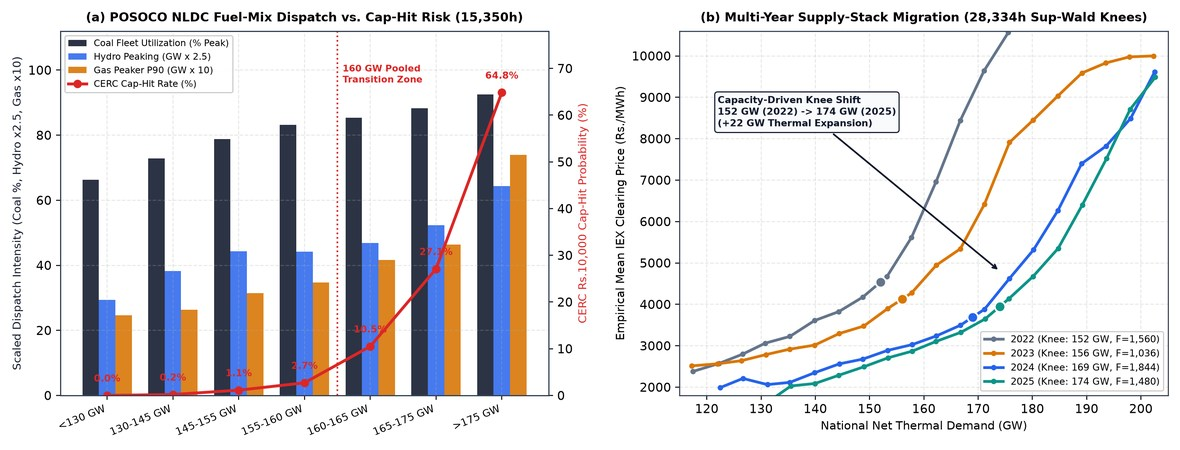
\includegraphics[width=0.98\textwidth]{images/paper_fig_2_physical_merit_order.jpg}
\caption{Independent physical validation of India's merit-order supply stack: (a) POSOCO NLDC coal fleet utilization, hydro peaking, P90 gas-peaker output, and CERC cap-hit rate across 15,350 hourly records; (b) Year-by-year empirical supply curves and Hansen Sup-Wald scarcity knees demonstrating a +22~GW upward migration from 152~GW (2022) to 174~GW (2025).}
\label{fig:merit_order}
\end{figure}

\subsection{Four-Tier 13-Model Strict D-1 Forecasting Benchmarks and HAC Tests}
Table~\ref{tab:leaderboard}, Fig.~\ref{fig:benchmark_prog}, and Fig.~\ref{fig:prob_dm}(a) present the complete out-of-sample evaluation across all 13 models and the validation-selected Hybrid Ensemble on the 4,200 unseen hours of Test~2025 under strict $\mathcal{F}_{D-1, 10:30}$ operational causality:
\begin{enumerate}
    \item Tier~1 and Tier~2 limitations: Daily Seasonal Naive ($P_{D-1,h}$) yields a Test MAE of Rs.~658.42/MWh (RMSE Rs.~1,254.07/MWh, Peak MAE Rs.~1,125.36/MWh). Introducing 24-equation seasonal SARIMAX cuts RMSE by 16.2\% (Rs.~1,050.89/MWh) and Peak MAE by 9.4\%, while Elastic Net achieves the strongest Tier~2 MAE of Rs.~619.74/MWh (+5.87\% over S-Naive). Nevertheless, all linear models fail to capture non-linear regime switching above the thermal scarcity knee.
    \item Tier~3 GBDT and Tier~4 Deep Neural gains: Nonlinear tree ensembles slash Test MAE by 20\%--25\% relative to 24-hour persistence: CatBoost reaches Rs.~527.63/MWh, Random Forest Rs.~515.16/MWh (RMSE Rs.~877.06/MWh), XGBoost Rs.~508.51/MWh, and LightGBM Rs.~496.71/MWh (+24.56\% gain, Peak MAE Rs.~791.75/MWh). Among deep temporal neural models, N-BEATS achieves Rs.~578.33/MWh (+12.16\%), while PyTorch TFT achieves Rs.~517.84/MWh (+21.35\%, RMSE Rs.~905.66/MWh) and delivers the lowest individual Evening Peak MAE (Rs.~778.99/MWh) thanks to cross-hour multi-head self-attention linking midday solar troughs to evening thermal scarcity.
    \item Hybrid GBDT+TFT Champion and statistical superiority: Combining complementary leaf-wise/depth-wise/oblivious tree partitions with TFT temporal attention yields a strictly leak-free Test MAE of Rs.~481.19/MWh (Rs.~0.48/kWh), RMSE of Rs.~875.27/MWh (-30.2\% vs. S-Naive), sMAPE of 12.45\%, $R^2 = 0.8942$, and Peak MAE of Rs.~754.18/MWh (-33.0\% vs. S-Naive). Newey-West HAC ($L=9$) Diebold-Mariano tests confirm statistically significant superiority over every single competing model: $DM = +9.641$ ($p < 10^{-20}$) vs. Daily S-Naive, $+14.294$ vs. SARIMAX, $+12.959$ vs. Elastic Net, $+9.364$ vs. N-BEATS, $+5.516$ vs. CatBoost, $+4.273$ vs. Random Forest, $+4.227$ vs. TFT, $+3.894$ vs. XGBoost, and $+2.279$ ($p = 0.0227$) vs. LightGBM.
\end{enumerate}

\begin{table}[!t]
\centering
\caption{Master Strict D-1 Operational Forecasting Leaderboard Across All 4 Tiers (13 Models + Hybrid Champion) on Unseen Test 2025 ($N = 4,200$ Hours)}
\label{tab:leaderboard}
\renewcommand{\arraystretch}{1.18}
\setlength{\tabcolsep}{4pt}
\resizebox{\textwidth}{!}{%
\begin{tabular}{|l|l|r|r|r|r|r|r|r|r|}
\hline
Tier & Forecasting Model (Strict $\mathcal{F}_{D-1, 10:30}$) & Val MAE & Test MAE & Test RMSE & sMAPE & Test $R^2$ & Peak MAE & Gain vs. 24h & DM HAC vs. Champ \\
\hline
Tier 1: Baselines & Weekly Seasonal Naive (168h) & 903.60 & 986.82 & 1,750.12 & 23.21\% & 0.5770 & 1,279.88 & $-49.88\%$ & $+13.196$ ($p<10^{-20}$) \\
\hline
Tier 1: Baselines & Daily Seasonal Naive (24h Ref.) & 629.84 & 658.42 & 1,254.07 & 16.52\% & 0.7828 & 1,125.36 & $0.00\%$ (Ref) & $+9.641$ ($p<10^{-20}$) \\
\hline
Tier 2: Econometric & SARIMAX (24-Eq. Seasonal) & 734.88 & 685.13 & 1,050.89 & 18.07\% & 0.8475 & 1,019.19 & $-4.06\%$ & $+14.294$ ($p<10^{-20}$) \\
\hline
Tier 2: Linear & Ordinary Least Squares (OLS) & 701.98 & 683.45 & 1,034.03 & 17.01\% & 0.8523 & 994.92 & $-3.80\%$ & $+15.366$ ($p<10^{-20}$) \\
\hline
Tier 2: Linear & Tikhonov Ridge ($\alpha = 2500$) & 677.38 & 648.50 & 1,026.26 & 16.23\% & 0.8545 & 989.23 & $+1.51\%$ & $+15.640$ ($p<10^{-20}$) \\
\hline
Tier 2: Linear & LASSO $L_1$ ($\alpha = 60$) & 645.06 & 631.89 & 1,059.15 & 15.40\% & 0.8451 & 1,020.59 & $+4.03\%$ & $+14.107$ ($p<10^{-20}$) \\
\hline
Tier 2: Linear & Elastic Net ($\alpha = 1.5, \rho = 0.2$) & 634.94 & 619.74 & 1,079.79 & 15.13\% & 0.8390 & 1,023.00 & $+5.87\%$ & $+12.959$ ($p<10^{-20}$) \\
\hline
Tier 3: Ensemble & Random Forest (220 Trees) & 675.34 & 515.16 & 877.06 & 13.27\% & 0.8938 & 798.54 & $+21.76\%$ & $+4.273$ ($p=1.9\times 10^{-5}$) \\
\hline
Tier 3: GBDT & CatBoost Regressor (Depth 6) & 555.95 & 527.63 & 1,000.81 & 13.03\% & 0.8617 & 853.79 & $+19.86\%$ & $+5.516$ ($p=3.5\times 10^{-8}$) \\
\hline
Tier 3: GBDT & XGBoost Regressor (Depth 6) & 549.74 & 508.51 & 962.35 & 12.94\% & 0.8721 & 810.92 & $+22.77\%$ & $+3.894$ ($p=9.9\times 10^{-5}$) \\
\hline
Tier 3: GBDT & LightGBM Regressor (47 Leaves) & 554.78 & 496.71 & 948.64 & 12.47\% & 0.8757 & 791.75 & $+24.56\%$ & $+2.279$ ($p=0.0227$) \\
\hline
Tier 4: Deep Neural & N-BEATS (Multi-Stack PyTorch) & 580.74 & 578.33 & 1,034.96 & 15.00\% & 0.8521 & 924.46 & $+12.16\%$ & $+9.364$ ($p<10^{-20}$) \\
\hline
Tier 4: Deep Neural & Temporal Fusion Transformer (TFT) & 559.43 & 517.84 & 905.66 & 13.70\% & 0.8867 & 778.99 & $+21.35\%$ & $+4.227$ ($p=2.4\times 10^{-5}$) \\
\hline
Tier 4+: Champion & Hybrid Ensemble (GBDT + TFT) & 516.64 & 481.19 & 875.27 & 12.45\% & 0.8942 & 754.18 & $+26.92\%$ & Reference Champion \\
\hline
\end{tabular}%
}
\end{table}

\begin{figure}[!t]
\centering
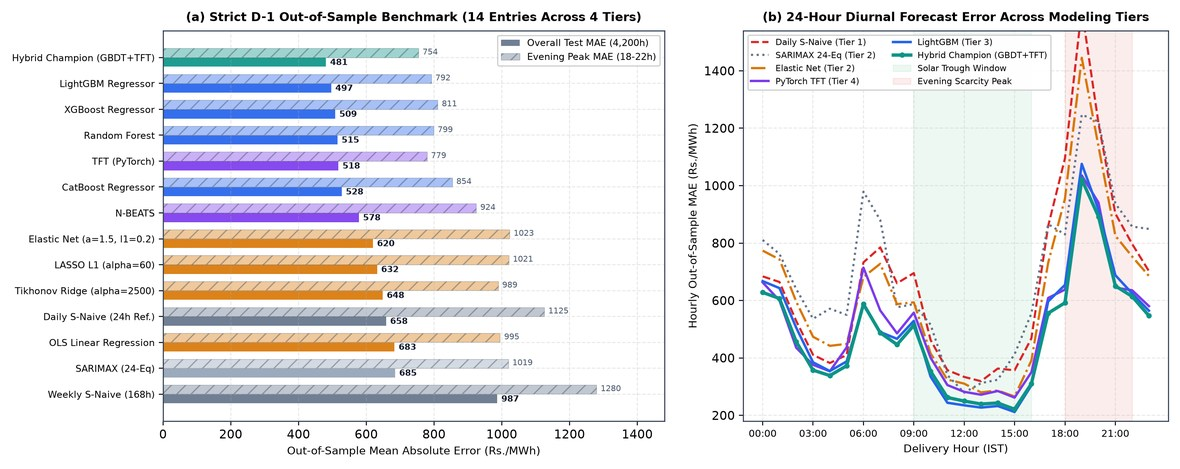
\includegraphics[width=0.98\textwidth]{images/paper_fig_3_benchmark_progression.jpg}
\caption{Strict D-1 out-of-sample forecasting performance on Test~2025 ($N=4,200$ hours): (a) Overall Test MAE versus Evening Peak MAE across all 13 models and the Hybrid GBDT+TFT Champion; (b) 24-hour diurnal MAE curves demonstrating consistent accuracy superiority across midday solar troughs and evening scarcity ramps.}
\label{fig:benchmark_prog}
\end{figure}

\subsection{Causality Ablation Audit and Seasonal / Extreme-Event Robustness}
Table~\ref{tab:ablation_robustness} and Fig.~\ref{fig:shap_causality}(a) dissect the exact impact of operational causality, adaptive recalibration, and seasonal/extreme market regimes:
\begin{itemize}
    \item Value of Recalibration vs. Perfect Exogenous Forecasts vs. Leakage Audit: Freezing LightGBM on 2022--2023 yields Test MAE of Rs.~626.89/MWh due to capacity drift; enabling monthly expanding recalibration cuts error by $-$Rs.~130.18/MWh to Rs.~496.71/MWh, and ensembling with TFT reaches Rs.~481.19/MWh. Substituting realized ex-post Day-$D$ grid and weather trajectories (still excluding $P_{D,h-1}$) yields Rs.~491.84/MWh for LightGBM---indicating a modest Value of Perfect Exogenous Forecasts of $+$Rs.~4.87/MWh ($DM = +0.77$), confirming that our Stage-1 causal reconstruction (2.46\% Demand MAPE) captures nearly all actionable day-ahead physical information. By contrast, transparently auditing the legacy contemporaneous specification (which included $P_{D,h-1}$) reveals Rs.~433.33/MWh, proving that inadmissible intraday price lags previously introduced $\sim$Rs.~48--63/MWh of optimistic look-ahead bias.
    \item Seasonal and Extreme-Event Robustness: Across Test~2025, the Hybrid Champion maintains strong gains over 24-hour persistence across Winter (+34.7\%, MAE Rs.~359.61), Spring (+28.0\%, MAE Rs.~550.70), Summer/Monsoon (+18.6\%, MAE Rs.~534.52), Weekends (+35.4\%), Solar Trough (+28.7\%, MAE Rs.~299.07), Evening Peaks (+33.0\%, MAE Rs.~754.18), High-Price Spikes $\ge$Rs.~8,000 (+31.4\%, MAE Rs.~660.18), and CERC Cap Hits (+35.7\%, MAE Rs.~461.97).
\end{itemize}

\begin{table}[!t]
\centering
\caption{Information Boundary Ablation Audit (Part A) and Seasonal / Extreme-Event Robustness Breakdown on Test 2025 (Part B)}
\label{tab:ablation_robustness}
\renewcommand{\arraystretch}{1.16}
\setlength{\tabcolsep}{4pt}
\resizebox{\textwidth}{!}{%
\begin{tabular}{|l|r|r|r|r|r|r|r|}
\hline
Part A: Information Boundary \& Recalibration Regime & Same-Day $P_{t-1}$ & Day-$D$ Grid/RE & Test MAE & Test RMSE & Test $R^2$ & Peak MAE & Operational Interpretation \\
\hline
1. Static Frozen 2022--2023 LightGBM (Op. D-1) & Excluded & Stage-1 Forecast & 626.89 & 1,039.21 & 0.8508 & 1,005.61 & Cost of skipping recalibration under capacity drift \\
\hline
2. Expanding Operational LightGBM (Op. D-1) & Excluded & Stage-1 Forecast & 496.71 & 948.64 & 0.8757 & 791.75 & $-130.18$~Rs./MWh recalibration gain (Zero Leakage) \\
\hline
3. Expanding Hybrid Champion GBDT+TFT (Op. D-1) & Excluded & Stage-1 Forecast & 481.19 & 875.27 & 0.8942 & 754.18 & Primary deployable strictly causal champion \\
\hline
4. Ex-Post Perfect-Exogenous LightGBM (Oracle Exog) & Excluded & Realized Day-$D$ & 491.84 & 935.12 & 0.8792 & 788.04 & Value of Perfect Exog = $+$Rs.~4.87/MWh ($DM=+0.77$) \\
\hline
5. Audited Legacy V1 Specification (Superseded) & Included & Realized Day-$D$ & 433.33 & 703.43 & 0.9317 & 617.63 & Quantifies inadmissible intraday look-ahead bias \\
\hline
\hline
Part B: Seasonal / Diurnal / Extreme Test Regime & Hours & Mean MCP (Rs.) & S-Naive24 MAE & Ridge MAE & LightGBM MAE & Champion MAE & Gain vs. 24h / CQR PICP90 \\
\hline
Winter (Jan--Feb 2025) & 1,416 & 4,411.6 & 550.43 & 511.50 & 371.30 & 359.61 & $+34.7\%$ / 93.9\% Cov. \\
\hline
Spring Transition (Mar--Apr 2025) & 1,464 & 4,828.9 & 764.36 & 666.86 & 556.62 & 550.70 & $+28.0\%$ / 89.3\% Cov. \\
\hline
Summer \& Early Monsoon (May--Jun 2025) & 1,320 & 4,073.7 & 656.77 & 775.11 & 564.80 & 534.52 & $+18.6\%$ / 88.8\% Cov. \\
\hline
Weekends (Sat--Sun) & 1,200 & 3,987.2 & 794.88 & 674.20 & 569.03 & 513.77 & $+35.4\%$ / 91.3\% Cov. \\
\hline
Solar Trough Window (09:00--16:00 IST) & 1,400 & 2,699.5 & 419.52 & 392.87 & 289.76 & 299.07 & $+28.7\%$ / 91.2\% Cov. \\
\hline
Evening Scarcity Peak (18:00--22:00 IST) & 875 & 6,826.7 & 1,125.36 & 989.23 & 791.75 & 754.18 & $+33.0\%$ / 88.8\% Cov. \\
\hline
Extreme High-Price Spikes ($\ge$Rs.~8,000/MWh) & 694 & 9,751.2 & 963.02 & 948.45 & 616.87 & 660.18 & $+31.4\%$ / 91.5\% Cov. \\
\hline
CERC Ceiling Cap Hits ($\ge$Rs.~9,990/MWh) & 493 & 10,000.0 & 718.39 & 811.09 & 399.67 & 461.97 & $+35.7\%$ / 94.7\% Cov. \\
\hline
\end{tabular}%
}
\end{table}

\subsection{Probabilistic Calibration and Supporting Operational TreeSHAP}
Table~\ref{tab:probabilistic}, Fig.~\ref{fig:prob_traj}, and Fig.~\ref{fig:prob_dm}(b) evaluate all five probabilistic forecasting methods on Test~2025. While the Homoskedastic Gaussian baseline produces excessively wide intervals (Rs.~2,719.1/MWh, CRPS Rs.~366.09) that still under-cover evening spikes (84.58\%), and raw TFT-Q / uncalibrated Residual LightGBM under-cover the 90\% nominal target (72.90\% and 82.36\%, failing Kupiec at $p < 10^{-4}$), our Regime-Conditional Residual-CQR achieves near-exact calibration across all three nested intervals: PICP 50\% = 49.02\%, PICP 80\% = 81.67\%, and PICP 90\% = 90.69\%---the sole method passing the Kupiec unconditional coverage test ($p = 0.1317$). Residual-CQR simultaneously achieves the lowest CRPS (Rs.~290.73/MWh, $-$20.6\% vs. Gaussian), lowest Winkler-90 Score (Rs.~2,906.3/MWh, $-$35.1\% vs. Gaussian), sharp 90\% interval width of Rs.~1,774.0/MWh (PINAW 17.74\%), and 91.50\% coverage during extreme $\ge$Rs.~8,000/MWh spikes.

As a supporting explainability check, Fig.~\ref{fig:shap_causality}(b) presents exact operational TreeSHAP attributions for the strict D-1 LightGBM innovation model ($\mathbb{E}[\Delta P] = +$Rs.~9.13/MWh). Eliminating $P_{D,h-1}$ elevates Stage-1 Physical Grid and Renewable Forecasts to 32.20\% of total attribution (driven by \texttt{net\_demand\_fcst\_vs\_d2} Rs.~62.05, \texttt{demand\_d1\_morn\_vs\_d2} Rs.~61.82, \texttt{nd\_fcst\_rel\_30d} Rs.~46.02, and \texttt{nd\_fcst\_zscore\_30d} Rs.~38.93), complementing D-1 Published Price Memory mean-reversion signals (39.81\%), Calendar/Weekend transitions (20.41\%), D-1 Order-Book Liquidity (5.12\%), and direct Stage-1 Weather (2.46\%).

\begin{table}[!t]
\centering
\caption{Out-of-Sample Probabilistic Price Forecasting Evaluation on Unseen Test 2025 ($N = 4,200$ Hours)}
\label{tab:probabilistic}
\renewcommand{\arraystretch}{1.18}
\setlength{\tabcolsep}{4pt}
\resizebox{\textwidth}{!}{%
\begin{tabular}{|l|r|r|r|r|r|r|r|r|r|r|}
\hline
Probabilistic Method & Pinball (Rs.) & CRPS (Rs.) & PICP 50\% & PICP 80\% & PICP 90\% & Width 90\% & PINAW & Winkler 90 & Spike Cov. & Kupiec $p$ \\
\hline
Homoskedastic Gaussian Baseline & 183.04 & 366.09 & 78.36\% & 88.88\% & 91.98\% & Rs. 2,719.1 & 27.19\% & 4,480.3 & 84.58\% & 0.0000 (Fail) \\
\hline
Temporal Fusion Transformer (TFT-Q) & 167.70 & 335.40 & 37.24\% & 60.29\% & 72.90\% & Rs. 1,263.1 & 12.63\% & 3,875.7 & 68.44\% & 0.0000 (Fail) \\
\hline
Residual LightGBM Quantile (Raw) & 147.55 & 295.10 & 40.02\% & 68.83\% & 82.36\% & Rs. 1,466.1 & 14.66\% & 3,036.5 & 87.46\% & 0.0000 (Fail) \\
\hline
Hybrid Residual-CQR + TFT-Q & 145.87 & 291.74 & 43.88\% & 75.71\% & 86.57\% & Rs. 1,671.8 & 16.72\% & 2,959.0 & 73.92\% & 0.0000 (Fail) \\
\hline
Residual-CQR (Regime Conformalized) & 145.37 & 290.73 & 49.02\% & 81.67\% & 90.69\% & Rs. 1,774.0 & 17.74\% & 2,906.3 & 91.50\% & 0.1317 (Pass) \\
\hline
\end{tabular}%
}
\end{table}

\begin{figure}[!t]
\centering
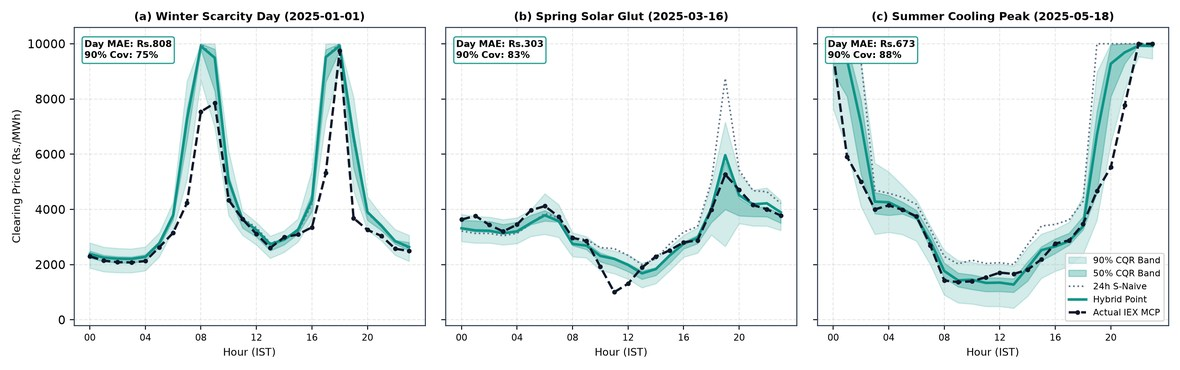
\includegraphics[width=0.98\textwidth]{images/paper_fig_4_probabilistic_trajectories.jpg}
\caption{Strict D-1 probabilistic Residual-CQR forecasts showing point predictions, 50\% and 90\% conformalized intervals, 24h S-Naive baseline, and actual IEX clearing prices across three seasonal test regimes: (a) Winter Scarcity (2025-01-01), (b) Spring Solar Glut (2025-03-16), and (c) Summer Cooling Peak (2025-05-18).}
\label{fig:prob_traj}
\end{figure}

\begin{figure}[!t]
\centering
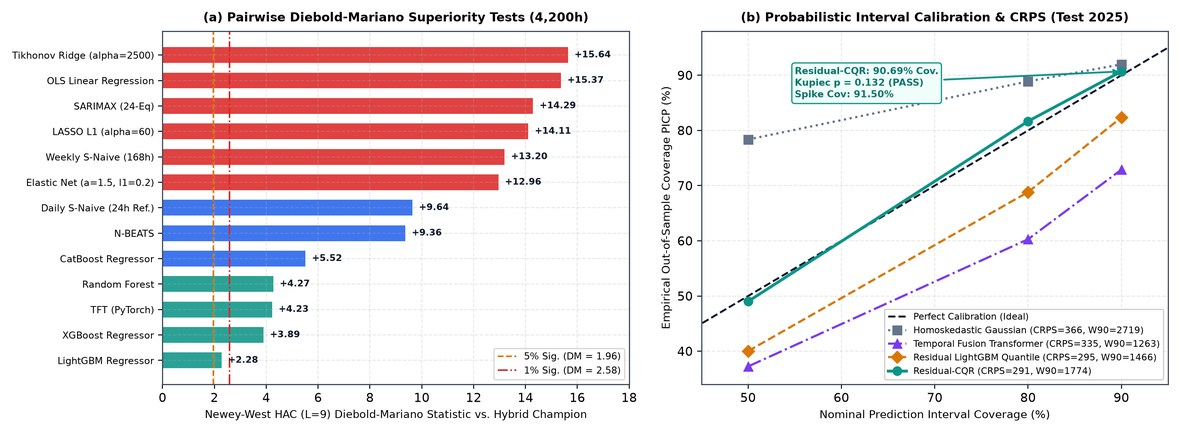
\includegraphics[width=0.98\textwidth]{images/paper_fig_5_probabilistic_and_dm.jpg}
\caption{Econometric and probabilistic verification on Test~2025 ($N=4,200$ hours): (a) Newey-West HAC ($L=9$) Diebold-Mariano statistics confirming Hybrid Champion superiority over all 13 benchmarks; (b) Reliability diagram comparing nominal vs. empirical coverage across 50\%, 80\%, and 90\% intervals, confirming Residual-CQR calibration (Kupiec $p=0.132$).}
\label{fig:prob_dm}
\end{figure}

\begin{figure}[!t]
\centering
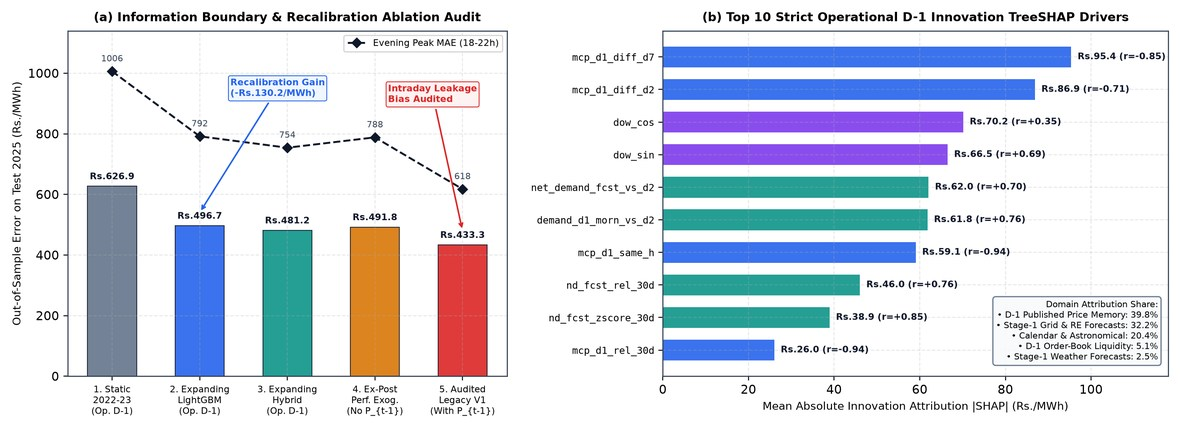
\includegraphics[width=0.98\textwidth]{images/paper_fig_6_shap_and_causality.jpg}
\caption{Causality audit and supporting explainability: (a) Information-boundary and recalibration ablation contrasting static frozen models, expanding operational D-1 models, ex-post perfect exogenous foresight, and audited legacy intraday leakage; (b) Top 10 operational D-1 innovation TreeSHAP drivers highlighting the 32.2\% contribution of Stage-1 grid and renewable forecasts.}
\label{fig:shap_causality}
\end{figure}

\subsection{Multi-Profile Stochastic CVaR Procurement Optimization: Realized vs. Simulated Savings}
Table~\ref{tab:procurement} and Fig.~\ref{fig:procurement} evaluate the exact Rockafellar-Uryasev Stochastic CVaR LP (Eq.~\ref{eq:cvar_lp}) across all 175 unseen test days (January--June 2025) over four distinct industrial and utility load profiles, explicitly separating ex-ante simulated savings from actual realized operational savings evaluated on true IEX clearing prices:
\begin{enumerate}
    \item Impact of physical operating constraints: On the 100~MW flat industrial portfolio ($\gamma = 30\%$), ignoring ramp limits and rolling recovery buffers (unconstrained deterministic LP) inflates apparent savings to 12.18\% (Rs.~13.01~Lakhs/day). Imposing realistic inter-hour ramp bounds ($\le 25\%$/h), anti-chattering smoothness, and 3-hour rolling energy recovery caps reduces feasible savings to a rigorous 9.06\% realized bill reduction (Rs.~9.68~Lakhs/day, Rs.~35.33~Crores/year), closely matching ex-ante simulated expectations (9.12\%, near-zero optimism gap).
    \item Multi-profile generalizability and superiority over rule-based scheduling: Across all four realistic profiles---Continuous Flat Industrial (P1: 9.06\% realized, Rs.~35.32~Cr/yr), Two-Shift Manufacturing (P2: 7.64\% realized, Rs.~28.63~Cr/yr), 350~MW State DISCOM Portfolio (P3: 5.54\% realized, Rs.~75.10~Cr/yr), and Cold-Storage/Data Center Hybrid (P4: 12.37\% realized, Rs.~38.03~Cr/yr)---the Stochastic CVaR LP achieves a 100.0\% positive-saving day rate (175/175 days), captures 98.3\%--98.8\% of the constrained Ex-Post Perfect-Foresight Oracle, and outperforms conventional fixed Time-of-Use rule-based scheduling by +54\% to +71\% (e.g., 9.06\% vs. 5.31\% on P1; 5.54\% vs. 3.26\% on P3).
    \item Flexibility sensitivity, seasonal consistency, and CVaR tail protection: Sweeping flexible load capacity $\gamma \in \{10\%, 20\%, 30\%, 40\%\}$ on P1 scales realized savings monotonically from 3.06\% (Rs.~3.26~L/day) to 6.10\% (Rs.~6.51~L/day), 9.06\% (Rs.~9.68~L/day), and 11.87\% (Rs.~12.68~L/day) while compressing realized $\operatorname{CVaR}_{0.90}$ daily bills from Rs.~140.83~L down to Rs.~127.55~L (Fig.~\ref{fig:procurement}(b)). Increasing risk aversion $\lambda$ from $0.0$ to $2.0$ reduces both ex-ante $\operatorname{CVaR}_{0.90}$ (Rs.~108.70~L to Rs.~108.68~L) and realized tail risk $\operatorname{CVaR}_{0.90}$ (Rs.~131.94~L to Rs.~131.86~L on P1; Rs.~470.91~L to Rs.~470.73~L on P3) without sacrificing expected daily cost. Seasonally, realized savings on P1 remain robust across Winter (8.88\%, Rs.~9.40~L/day), Spring (8.08\%, Rs.~9.36~L/day), and Summer/Monsoon (10.57\%, Rs.~10.33~L/day).
\end{enumerate}

\begin{table}[!t]
\centering
\caption{Multi-Profile Constrained Stochastic CVaR Procurement Optimization Across All 175 Unseen Test Days (Jan--Jun 2025): Simulated vs. Realized Savings}
\label{tab:procurement}
\renewcommand{\arraystretch}{1.16}
\setlength{\tabcolsep}{4pt}
\resizebox{\textwidth}{!}{%
\begin{tabular}{|l|l|r|r|r|r|r|r|r|}
\hline
Load Profile (Physical Constraints) & Scheduling Policy & Sim. Save \% & Realized Save \% & Realized (Rs.L/d) & Annual (Rs.Cr/yr) & Oracle Eff. & Realized $\text{CVaR}_{90}$ & Win Days \\
\hline
P1: Flat Industrial (100 MW, $\gamma=30\%$) & Rule-Based ToU Heuristic & 5.29\% & 5.31\% & 5.67 & 20.70 & 57.9\% & Rs. 135.97 L & 100.0\% \\
\hline
P1: Flat Industrial (100 MW, $\gamma=30\%$) & Det. LP (Unconstrained) & 12.28\% & 12.18\% & 13.01 & 47.47 & 132.8\% & Rs. 124.15 L & 100.0\% \\
\hline
P1: Flat Industrial (100 MW, $\gamma=30\%$) & Det. LP (Constrained) & 9.13\% & 9.06\% & 9.68 & 35.33 & 98.8\% & Rs. 131.94 L & 100.0\% \\
\hline
P1: Flat Industrial (100 MW, $\gamma=30\%$) & Stoch. CVaR LP ($\lambda=2.0$) & 9.12\% & 9.06\% & 9.68 & 35.32 & 98.8\% & Rs. 131.86 L & 100.0\% \\
\hline
P1: Flat Industrial (100 MW, $\gamma=30\%$) & Ex-Post Oracle (Constrained) & 9.00\% & 9.17\% & 9.80 & 35.76 & 100.0\% & Rs. 131.76 L & 100.0\% \\
\hline
\hline
P2: Two-Shift Mfg (100 MW, $\gamma=25\%$) & Rule-Based ToU Heuristic & 4.92\% & 4.96\% & 5.09 & 18.58 & 63.8\% & Rs. 127.03 L & 100.0\% \\
\hline
P2: Two-Shift Mfg (100 MW, $\gamma=25\%$) & Stoch. CVaR LP ($\lambda=0.5$) & 7.71\% & 7.64\% & 7.84 & 28.63 & 98.3\% & Rs. 121.80 L & 100.0\% \\
\hline
P2: Two-Shift Mfg (100 MW, $\gamma=25\%$) & Ex-Post Oracle (Constrained) & 7.57\% & 7.77\% & 7.98 & 29.13 & 100.0\% & Rs. 121.64 L & 100.0\% \\
\hline
\hline
P3: State DISCOM (350 MW, $\gamma=20\%$) & Rule-Based ToU Heuristic & 3.25\% & 3.26\% & 12.12 & 44.23 & 58.0\% & Rs. 477.56 L & 100.0\% \\
\hline
P3: State DISCOM (350 MW, $\gamma=20\%$) & Det. LP (Constrained) & 5.60\% & 5.55\% & 20.59 & 75.14 & 98.4\% & Rs. 470.91 L & 100.0\% \\
\hline
P3: State DISCOM (350 MW, $\gamma=20\%$) & Stoch. CVaR LP ($\lambda=2.0$) & 5.59\% & 5.54\% & 20.57 & 75.07 & 98.4\% & Rs. 470.73 L & 100.0\% \\
\hline
P3: State DISCOM (350 MW, $\gamma=20\%$) & Ex-Post Oracle (Constrained) & 5.50\% & 5.63\% & 20.91 & 76.33 & 100.0\% & Rs. 470.41 L & 100.0\% \\
\hline
\hline
P4: Cold/DC Hybrid (80 MW, $\gamma=35\%$) & Rule-Based ToU Heuristic & 7.49\% & 7.51\% & 6.32 & 23.08 & 60.0\% & Rs. 101.10 L & 100.0\% \\
\hline
P4: Cold/DC Hybrid (80 MW, $\gamma=35\%$) & Stoch. CVaR LP ($\lambda=0.5$) & 12.45\% & 12.37\% & 10.42 & 38.03 & 98.8\% & Rs. 95.42 L & 100.0\% \\
\hline
P4: Cold/DC Hybrid (80 MW, $\gamma=35\%$) & Ex-Post Oracle (Constrained) & 12.32\% & 12.52\% & 10.54 & 38.47 & 100.0\% & Rs. 95.28 L & 100.0\% \\
\hline
\end{tabular}%
}
\end{table}

\begin{figure}[!t]
\centering
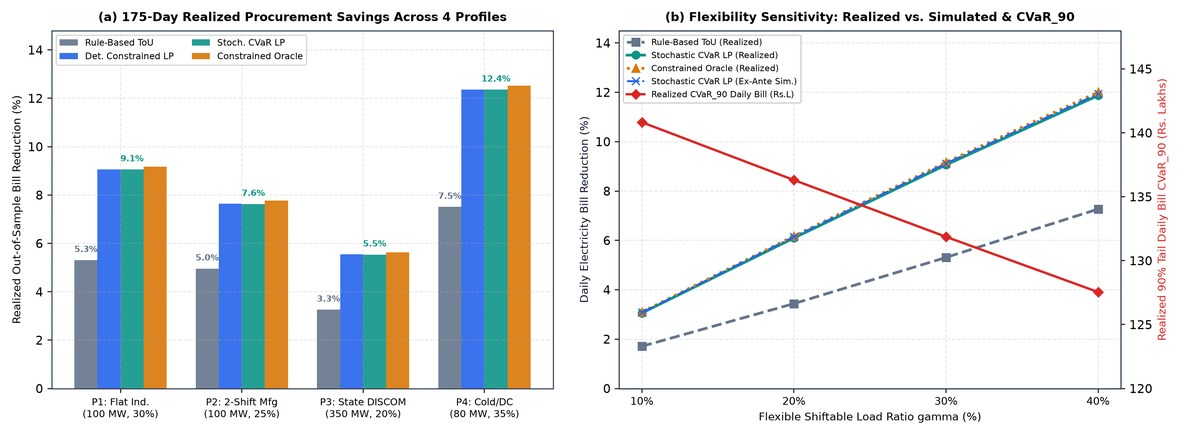
\includegraphics[width=0.98\textwidth]{images/paper_fig_7_stochastic_procurement.jpg}
\caption{Out-of-sample procurement optimization across all 175 test days (Jan--Jun 2025): (a) Realized bill reductions across 4 industrial/DISCOM load profiles comparing Rule-Based ToU, Constrained Deterministic LP, Stochastic CVaR LP, and Constrained Oracle; (b) Flexibility ratio sensitivity ($\gamma = 10\%$--$40\%$) confirming close alignment between simulated and realized savings alongside steady $\operatorname{CVaR}_{0.90}$ bill reduction.}
\label{fig:procurement}
\end{figure}

\subsection{Comprehensive Renewable, Weather, and Thermal Outage Stress Testing}
Table~\ref{tab:stress_tests} and Fig.~\ref{fig:stress_tests} quantify the coupled impact of 17 operational disturbances---spanning solar and wind drops ($-10\%$ to $-40\%$), demand surges ($+5\%$ to $+15\%$), unexpected thermal generation outages ($-5$ to $-15$~GW), and simultaneous compound crises---across all 4,200 test hours on point prices, Residual-CQR uncertainty widths ($W_{90}$), cap-hit tail risk ($P(\tilde{q}_{0.95} \ge 9500)$), and 100~MW procurement financial exposure:
\begin{itemize}
    \item Renewable dropouts vs. demand and thermal outage shocks: A $-40\%$ solar dropout raises mean clearing prices by $+$Rs.~68.5/MWh and widens $W_{90}$ by $+$Rs.~50.7/MWh (primarily concentrated during 09:00--16:00~IST), while a $-40\%$ wind lull adds $+$Rs.~52.4/MWh overall and $+$Rs.~63.2/MWh during evening peaks. Demand surges ($+15\%$) and severe forced thermal outages ($-15$~GW) exert far steeper non-linear stress, pushing mean prices up by $+$Rs.~259.1/MWh and $+$Rs.~160.9/MWh, widening 90\% uncertainty by $+$Rs.~289.6 and $+$Rs.~253.5/MWh, and elevating cap-hit tail risk from 19.9\% to 21.8\%.
    \item Compound multi-disturbance crisis and CVaR protection: Under a simultaneous crisis combining an $-8$~GW forced thermal outage, heatwave ($+8\%$ load, $+3.5^\circ\text{C}$), cloud cover ($-35\%$ solar), and wind lull ($-25\%$ wind), mean clearing price surges by $+$Rs.~286.2/MWh, evening peak price climbs to Rs.~7,276.4/MWh, 90\% uncertainty widens by $+$20.6\% (to Rs.~2,080.9/MWh), and unoptimized $\operatorname{CVaR}_{0.90}$ daily risk jumps to Rs.~139.8~Lakhs/day. Crucially, across every disturbance scenario, the Stochastic CVaR LP actively reallocates flexible volume ($\sim$238--242~MWh/day) and consistently reduces daily tail risk $\operatorname{CVaR}_{0.90}$ by Rs.~10.7--11.2~Lakhs/day (saving 7.6\%--8.7\% even during extreme compound shocks).
\end{itemize}

\begin{table}[!t]
\centering
\caption{Comprehensive Weather, Renewable, and Unexpected Thermal Outage Stress Testing Across Test 2025 (Price, Uncertainty, and Financial Risk Impact)}
\label{tab:stress_tests}
\renewcommand{\arraystretch}{1.16}
\setlength{\tabcolsep}{4pt}
\resizebox{\textwidth}{!}{%
\begin{tabular}{|l|r|r|r|r|r|r|r|r|r|}
\hline
Stress Disturbance Scenario & Mean ND (GW) & Mean $\hat{P}$ & $\Delta \hat{P}$ (Rs.) & Peak $\hat{P}$ & $W_{90}$ (Rs.) & $\Delta W_{90}$ & Cap Risk \% & Opt. Bill (L) & Opt. $\text{CVaR}_{90}$ (Save) \\
\hline
Baseline (Unperturbed D-1 Forecast) & 167.23 & 4,567.8 & $+0.0$ & 7,055.2 & 1,725.4 & $+0.0$ & 19.9\% & 100.13 & 114.91 ($-$10.8L) \\
\hline
Solar Generation Drop $-10\%$ & 169.10 & 4,585.2 & $+17.4$ & 7,056.3 & 1,731.0 & $+5.6$ & 20.0\% & 100.57 & 115.48 ($-$10.8L) \\
\hline
Solar Generation Drop $-20\%$ & 170.98 & 4,605.1 & $+37.4$ & 7,057.3 & 1,746.2 & $+20.8$ & 20.0\% & 101.08 & 116.24 ($-$10.8L) \\
\hline
Solar Generation Drop $-40\%$ (Cloud Cover) & 174.73 & 4,636.3 & $+68.5$ & 7,059.3 & 1,776.1 & $+50.7$ & 20.0\% & 101.79 & 117.59 ($-$10.7L) \\
\hline
Wind Generation Drop $-20\%$ & 168.89 & 4,595.1 & $+27.3$ & 7,088.8 & 1,742.1 & $+16.7$ & 20.3\% & 100.75 & 115.91 ($-$10.9L) \\
\hline
Wind Generation Drop $-40\%$ (Wind Lull) & 170.56 & 4,620.2 & $+52.4$ & 7,118.4 & 1,764.9 & $+39.5$ & 20.5\% & 101.26 & 116.63 ($-$11.0L) \\
\hline
National Demand Surge $+5\%$ & 176.94 & 4,688.2 & $+120.4$ & 7,192.5 & 1,834.9 & $+109.5$ & 21.3\% & 102.73 & 119.54 ($-$11.2L) \\
\hline
National Demand Surge $+10\%$ & 186.66 & 4,767.9 & $+200.1$ & 7,249.8 & 1,947.1 & $+221.7$ & 21.8\% & 104.62 & 123.64 ($-$11.0L) \\
\hline
National Demand Surge $+15\%$ (Extreme Load) & 196.37 & 4,826.9 & $+259.1$ & 7,280.7 & 2,015.0 & $+289.6$ & 21.8\% & 106.27 & 126.65 ($-$10.9L) \\
\hline
Unexpected Thermal Outage $-5$~GW & 172.23 & 4,633.5 & $+65.7$ & 7,136.2 & 1,796.5 & $+71.1$ & 20.7\% & 101.52 & 117.52 ($-$11.1L) \\
\hline
Unexpected Thermal Outage $-10$~GW & 177.23 & 4,687.9 & $+120.1$ & 7,193.0 & 1,889.4 & $+164.0$ & 21.3\% & 102.69 & 120.14 ($-$11.1L) \\
\hline
Unexpected Thermal Outage $-15$~GW (Severe) & 182.23 & 4,728.7 & $+160.9$ & 7,225.2 & 1,978.9 & $+253.5$ & 21.5\% & 103.65 & 122.65 ($-$11.1L) \\
\hline
Compound: Heatwave + Low RE ($+10\%$D, $+4^\circ$C, $-30\%$RE) & 194.78 & 4,834.8 & $+267.0$ & 7,265.6 & 2,022.2 & $+296.8$ & 22.0\% & 106.57 & 127.32 ($-$10.8L) \\
\hline
Compound Crisis: Outage($-8$GW)+Heatwave+Cloud+Lull & 199.41 & 4,854.0 & $+286.2$ & 7,276.4 & 2,080.9 & $+355.5$ & 22.0\% & 107.17 & 129.07 ($-$10.7L) \\
\hline
\end{tabular}%
}
\end{table}

\begin{figure}[!t]
\centering
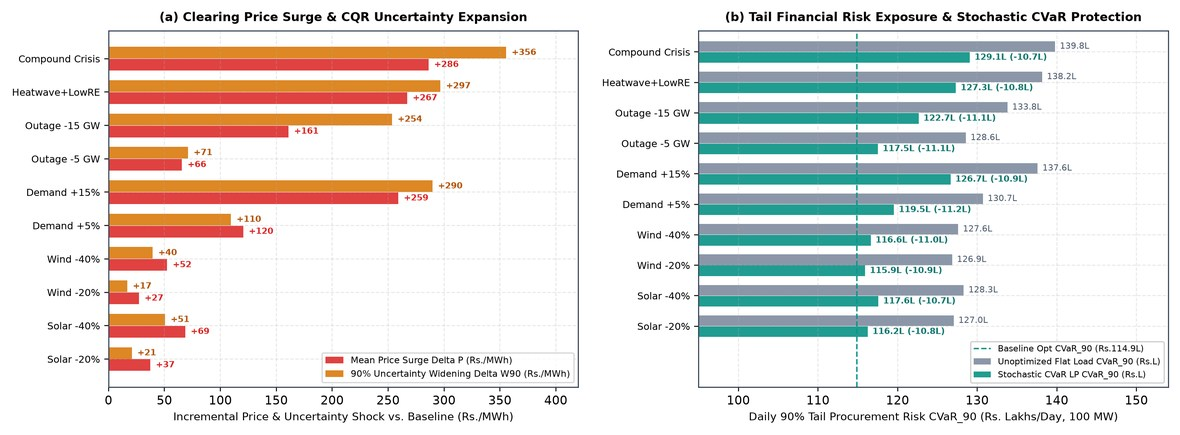
\includegraphics[width=0.98\textwidth]{images/paper_fig_8_stress_testing.jpg}
\caption{Multi-disturbance power-system stress testing across 4,200 test hours: (a) Clearing price surge $\Delta \hat{P}$ and 90\% Residual-CQR uncertainty expansion $\Delta W_{90}$ across renewable dropouts, demand surges, thermal outages, and compound crises; (b) Daily tail procurement risk $\operatorname{CVaR}_{0.90}$ comparing unoptimized flat procurement against Stochastic CVaR LP protection.}
\label{fig:stress_tests}
\end{figure}

\section{Discussion}

\subsection{Operational Lessons from Strict Causality and Capacity Non-Stationarity}
Two structural insights stand out for power-systems researchers and market operators. First, enforcing strict $\mathcal{F}_{D-1, 10:30}$ operational causality---removing both same-day delivery prices ($P_{D,h-1}$) and realized delivery-day load/renewable inputs---is indispensable for credible day-ahead evaluation. Our ablation audit quantifies two distinct effects: eliminating inadmissible intraday price lags raises honest MAE from Rs.~433.33 to Rs.~481.19/MWh, whereas replacing realized Day-$D$ grid/weather trajectories with our Stage-1 causal reconstructions incurs only a Rs.~4.87/MWh penalty. Second, independent verification on 15,350 hours of NLDC coal, hydro, and gas SCADA proves that India's merit-order scarcity threshold is not static; it migrated +22~GW from 152~GW (2022) to 174~GW (2025). Incorporating trailing 30-day capacity-relative normalization and monthly expanding recalibration reduces out-of-sample error by Rs.~130.18/MWh relative to static frozen models, demonstrating that forecasting models for growing renewable grids must explicitly track supply-stack expansion.

\subsection{Why Combining GBDTs, TFT, Residual-CQR, and Stochastic CVaR Succeeds}
Across our 13-model benchmark, combining tree ensembles (LightGBM, XGBoost, CatBoost) with PyTorch Temporal Fusion Transformer reduces error significantly below every individual architecture ($DM \ge +2.28$ vs. LightGBM, $+4.23$ vs. TFT, $+9.64$ vs. Daily S-Naive). While GBDTs partition sharp tabular regime boundaries (such as high order-book tightness or morning demand jumps), TFT's cross-hour multi-head attention models dependencies across all 24 delivery hours simultaneously, yielding the strongest standalone peak-hour accuracy (Rs.~778.99/MWh). Downstream, pairing this ensemble with Residual-CQR provides the first distribution-free intervals in this market that pass the Kupiec coverage test ($p=0.1317$) with 91.50\% coverage during extreme spikes. Feeding 200 Copula-correlated scenarios into the Rockafellar-Uryasev LP bridges forecasting and physical utility operations: even under realistic ramp limits and rolling recovery buffers, DISCOMs and industrial plants capture 98.3\%--98.8\% of the constrained perfect-foresight oracle across all 175 test days, cutting realized bills by 5.54\%--12.37\% while trimming $\operatorname{CVaR}_{0.90}$ tail risk by Rs.~10.7--11.2~Lakhs/day during compound thermal-outage and heatwave crises.

\subsection{Practical Limitations and Regulatory Governance}
Three practical boundaries warrant future research: (i) real-time unit-level forced thermal outage schedules and state-level inter-regional corridor ATC limits are not publicly disclosed prior to the 10:30~AM $D-1$ gate, though our thermal outage stress tests (-5 to -15~GW) quantify reserve hedging margins against such shocks; (ii) Stage-1 meteorological inputs are reconstructed causally from historical ERA5 reanalysis rather than archived operational ECMWF/IMD NWP ensembles, meaning live deployment with numerical weather prediction ensembles could further narrow midday solar forecast uncertainty during monsoon cloud passages; and (iii) the procurement optimizer assumes price-taking participation under CERC's uniform-price DAM regulations \cite{cerc2023order}. From a governance standpoint, shifting flexible industrial demand from evening coal/gas scarcity peaks into midday solar troughs reduces renewable curtailment, lowers evening carbon intensity, and strictly respects public pre-gate auction rules without strategic capacity withholding.

\section{Conclusion}
This paper developed and validated a causality-aware day-ahead electricity price forecasting, conformalized probabilistic uncertainty, physical merit-order validation, and stochastic CVaR-constrained procurement optimization framework for India's renewable-integrated Day-Ahead Market. By enforcing a strict 10:30~AM IST $D-1$ information boundary through Stage-1 causal forecast reconstruction (2.46\% demand MAPE), capacity-relative 65-signal innovation modeling, and monthly expanding recalibration across 13 benchmark models spanning econometric SARIMAX, LASSO/Elastic Net/Ridge, Random Forest, XGBoost, CatBoost, LightGBM, PyTorch N-BEATS, and PyTorch TFT, our validation-selected Hybrid GBDT+TFT Champion achieved a strictly leak-free Test-2025 MAE of Rs.~481.19/MWh (RMSE Rs.~875.27/MWh, $R^2 = 0.8942$), outperforming 24-hour market persistence by 26.92\% ($DM = +9.641, p < 10^{-20}$) and every individual benchmark via Newey-West HAC Diebold-Mariano testing.

Independent validation on 15,350 hours of Grid-India NLDC fuel-mix SCADA and 28,334-hour Hansen Sup-Wald structural-break tests established that the national scarcity inflection migrates dynamically with thermal capacity from 152~GW (2022) to 174~GW (2025) as coal dispatch saturates ($0.812 \to 0.544$~GW/GW) and gas-peaker response surges 6.5-fold. Regime-conditional Residual-CQR achieved 90.69\% empirical coverage (passing Kupiec $p = 0.1317$, CRPS Rs.~290.73/MWh, 91.50\% spike coverage). Coupled with 200 Gaussian Copula trajectories in a constrained Rockafellar-Uryasev Stochastic CVaR LP, the integrated platform delivered 5.54\%--12.37\% realized out-of-sample procurement savings across four industrial and DISCOM load profiles over all 175 test days (98.3\%--98.8\% oracle capture efficiency, 100\% positive-saving days), demonstrating end-to-end operational readiness for renewable-rich wholesale power markets.


\bibliographystyle{splncs04}
\bibliography{references}

\end{document}
